%%%%%%%%%%%%%%%%%%%%%%%%%%%%%%%%%%%%%%%%%%%%%%%%%%%%%%%%%%%%%%%%%%%%%%%%%%%%%%%%%%
\begin{frame}[fragile]\frametitle{}
\begin{center}
{\Large Decision Tree}
\end{center}
\end{frame}


%%%%%%%%%%%%%%%%%%%%%%%%%%%%%%%%%%%%%%%%%%%%%%%%%%%%%%%%%%%%%%%%%%%%%%%%%%%%%%%%%%
\begin{frame}[fragile]\frametitle{}
\begin{center}
{\Large Lets play a game}
\end{center}
\end{frame}


%%%%%%%%%%%%%%%%%%%%%%%%%%%%%%%%%%%%%%%%%%%%%%%%%%%%%%%%%%%%%%%%%%%%%%%%
\begin{frame}[fragile]\frametitle{Game}
Remember `20 questions' game?
\begin{itemize}
	\item Some one holds name of one famous person in mind
	\item Others need to find out that by asking, at max, 20 questions.
	\item Questions should be such that the answers to which are only Yes or No.
	\item No queries, no descriptive answers, nothing else.
	\end{itemize}
\end{frame}

%%%%%%%%%%%%%%%%%%%%%%%%%%%%%%%%%%%%%%%%%%%%%%%%%%%%%%%%%%%%%%%%%%%%%%%%
\begin{frame}[fragile]\frametitle{Game}
What are we doing here, essentially?
\begin{itemize}
	\item Eliminating subgroups.
	\item So, for question `Male or Female', any answer will remove half of the population from our search space.
	\item Each of these questions are actually splitting the search space one by one.
	\item Making it narrower and narrower.
	\item Till we get to one person.
	\end{itemize}
\end{frame}

%%%%%%%%%%%%%%%%%%%%%%%%%%%%%%%%%%%%%%%%%%%%%%%%%%%%%%%%%%%%%%%%%%%%%%%%
\begin{frame}[fragile]\frametitle{Game}
Its a tree.
\begin{itemize}
	\item Starting at root
	\item Each question at node
	\item Answer at leaves
	\item Whats the max depth of the tree allowed in the game we just discussed?
	\end{itemize}
\end{frame}

%%%%%%%%%%%%%%%%%%%%%%%%%%%%%%%%%%%%%%%%%%%%%%%%%%%%%%%%%%%%%%%%%%%%%%%%
\begin{frame}[fragile]\frametitle{Game}
Whats the success?
\begin{itemize}
	\item Idea is to have minimum depth ie minimum number of questions
	\item So, your questions should be such that you get to the answer quicker.
	\end{itemize}
This is the decision tree, and the questions or the splits decides its success.
\end{frame}

%%%%%%%%%%%%%%%%%%%%%%%%%%%%%%%%%%%%%%%%%%%%%%%%%%%%%%%%%%%%%%%%%%%%%%%%
\begin{frame}[fragile]\frametitle{Tree? - Comp Science way}
\begin{itemize}
	\item What is a Tree?
	\item Comp Science definition?
	\item What are other Data Structures?
	\item Diff between Tree and Graph?
	\end{itemize}
\end{frame}

%%%%%%%%%%%%%%%%%%%%%%%%%%%%%%%%%%%%%%%%%%%%%%%%%%%%%%%%%%%%%%%%%%%%%%%%%%%%%%%%%%
\begin{frame}[fragile]\frametitle{}
\begin{center}
{\Large Decision Tree Example - Admissions}
\end{center}
\end{frame}

%%%%%%%%%%%%%%%%%%%%%%%%%%%%%%%%%%%%%%%%%%%%%%%%%%%%%%%%%%%%%%%%%%%%%%%%
\begin{frame}[fragile]\frametitle{Admissions}
\begin{itemize}
	\item Admission to a reputed college depends, say, on JEE score as well as 12th std marks.
	\item Previous data of 1000 applicants shows that average JEE score for admitted students is 150 and average 12th std marks are 80\%. 
	\item We are asked to create a model that will allow us to predict students most likely to be admitted. 
	\item How do we go about doing this?
	\end{itemize}
\end{frame}

%%%%%%%%%%%%%%%%%%%%%%%%%%%%%%%%%%%%%%%%%%%%%%%%%%%%%%%%%%%%%%%%%%%%%%%%
\begin{frame}[fragile]\frametitle{Approach}
\begin{itemize}
	\item Divide applicants into subgroups: those with more than, say, like 130 JEE, are in 'more likely' group
	\item Draw the tree
	\end{itemize}

\end{frame}

%%%%%%%%%%%%%%%%%%%%%%%%%%%%%%%%%%%%%%%%%%%%%%%%%%%%%%%%%%
\begin{frame}[fragile]\frametitle{Approach}
\begin{center}
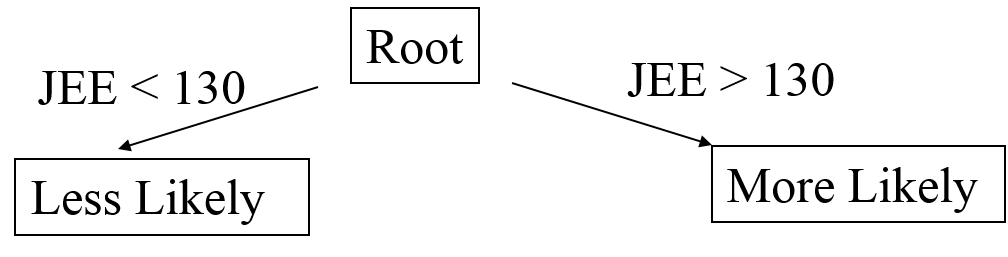
\includegraphics[width=0.7\linewidth,keepaspectratio]{treeex1}
\end{center}
\end{frame}


%%%%%%%%%%%%%%%%%%%%%%%%%%%%%%%%%%%%%%%%%%%%%%%%%%%%%%%%%%%%%%%%%%%%%%%%
\begin{frame}[fragile]\frametitle{Approach}
\begin{itemize}
	\item Split this group itself based 12th percentage, above 70\% (called ``most likely'') or below (called ``high maybe'').
	\item Add to the tree
	\end{itemize}

\end{frame}

%%%%%%%%%%%%%%%%%%%%%%%%%%%%%%%%%%%%%%%%%%%%%%%%%%%%%%%%%%
\begin{frame}[fragile]\frametitle{Approach}
\begin{center}
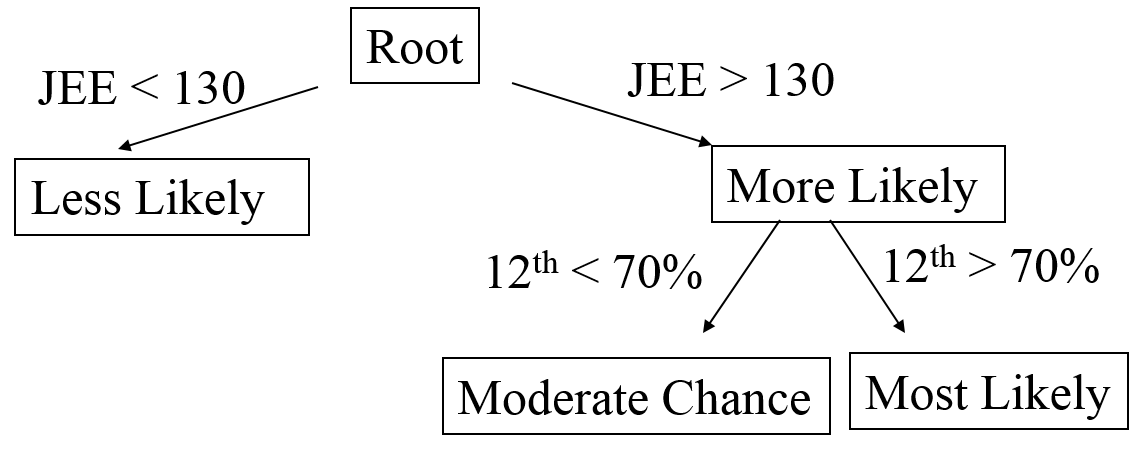
\includegraphics[width=0.7\linewidth,keepaspectratio]{treeex2}
\end{center}
\end{frame}


%%%%%%%%%%%%%%%%%%%%%%%%%%%%%%%%%%%%%%%%%%%%%%%%%%%%%%%%%%%%%%%%%%%%%%%%
\begin{frame}[fragile]\frametitle{Approach}
\begin{itemize}
	\item Then we do the same thing to the group with JEE score below 130, calling these subgroups as ``Less Likely''.
	\item Add to the tree and finish till the leaves.
	\end{itemize}

\end{frame}

%%%%%%%%%%%%%%%%%%%%%%%%%%%%%%%%%%%%%%%%%%%%%%%%%%%%%%%%%%%%%%%%%%%%%%%%
\begin{frame}[fragile]\frametitle{Approach}
\begin{itemize}
	\item We thus formed a Decision Tree.
	\item We can now predict outcome of any unknown case.
	\end{itemize}

\end{frame}

%%%%%%%%%%%%%%%%%%%%%%%%%%%%%%%%%%%%%%%%%%%%%%%%%%%%%%%%%%%%%%%%%%%%%%%%
\begin{frame}[fragile]\frametitle{Questions}
\begin{itemize}
	\item What if we split on 12th marks first and then JEE scores - would we get the same groupings? 
	\item What is the best way to split?
	\end{itemize}
\end{frame}

%%%%%%%%%%%%%%%%%%%%%%%%%%%%%%%%%%%%%%%%%%%%%%%%%%%%%%%%%%%%%%%%%%%%%%%%
\begin{frame}[fragile]\frametitle{Questions}
\begin{itemize}
	\item What if we used more criteria such as essay evaluation scores, extra curricular, awards and distinctions in sports etc. i.e. how many attributes should we use to create splits and what are the most significant attributes.
	\end{itemize}
All these criteria can be modeled using Decision Tree technique.
\end{frame}

%%%%%%%%%%%%%%%%%%%%%%%%%%%%%%%%%%%%%%%%%%%%%%%%%%%%%%%%%%%%%%%%%%%%%%%%%%%%%%%%%%
\begin{frame}[fragile]\frametitle{}
\begin{center}
{\Large Decision Tree in Machine Learning}
\end{center}
\end{frame}


% %%%%%%%%%%%%%%%%%%%%%%%%%%%%%%%%%%%%%%%%%%%%%%%%%%%%%%%%%%%%%%%%%%%%%%%%
% \begin{frame}[fragile]\frametitle{Decision Trees}
% \begin{itemize}
	% \item  It works for both categorical and continuous dependent variables.
	% \item In this algorithm, we split the population into two or more homogeneous sets. 
	% \item This is done based on most significant attributes/ independent variables to make as distinct groups as possible.
	% \item E.g. There could be many reasons for a cricket match to happen or cancel: rains, sunny, overcast, etc.
	% \end{itemize}
% \end{frame}

% %%%%%%%%%%%%%%%%%%%%%%%%%%%%%%%%%%%%%%%%%%%%%%%%%%%%%%%%%%
% \begin{frame}[fragile]\frametitle{Decision Trees}
% \begin{center}
% 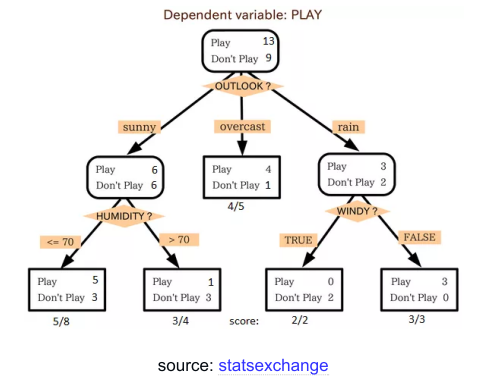
\includegraphics[width=\linewidth,keepaspectratio]{play}
% \end{center}
% \end{frame}

%%%%%%%%%%%%%%%%%%%%%%%%%%%%%%%%%%%%%%%%%%%%%%%%%%%%%%%%%%%%%%%%%%%%%%%%
\begin{frame}[fragile]\frametitle{Decision Trees}
\begin{itemize}
	\item  Decision Trees (DTs) are a non-linear supervised learning method used for classification and regression. 
	\item The goal is to create a model that predicts the value of a target variable by learning simple decision rules inferred from the data features.
%\item A decision tree is a simple representation for classifying examples. 
%\item Decision tree learning is one of the most successful techniques for supervised classification learning [citation needed].
	\end{itemize}
\end{frame}

%%%%%%%%%%%%%%%%%%%%%%%%%%%%%%%%%%%%%%%%%%%%%%%%%%%%%%%%%%%%%%%%%%%%%%%%
\begin{frame}[fragile]\frametitle{Decision Trees}
Can you rewrite the previous decision trees as a If-then-else statement?

\end{frame}

%%%%%%%%%%%%%%%%%%%%%%%%%%%%%%%%%%%%%%%%%%%%%%%%%%%%%%%%%%%%%%%%%%%%%%%%
\begin{frame}[fragile]\frametitle{Graphically}
Decision Boundaries
\begin{center}
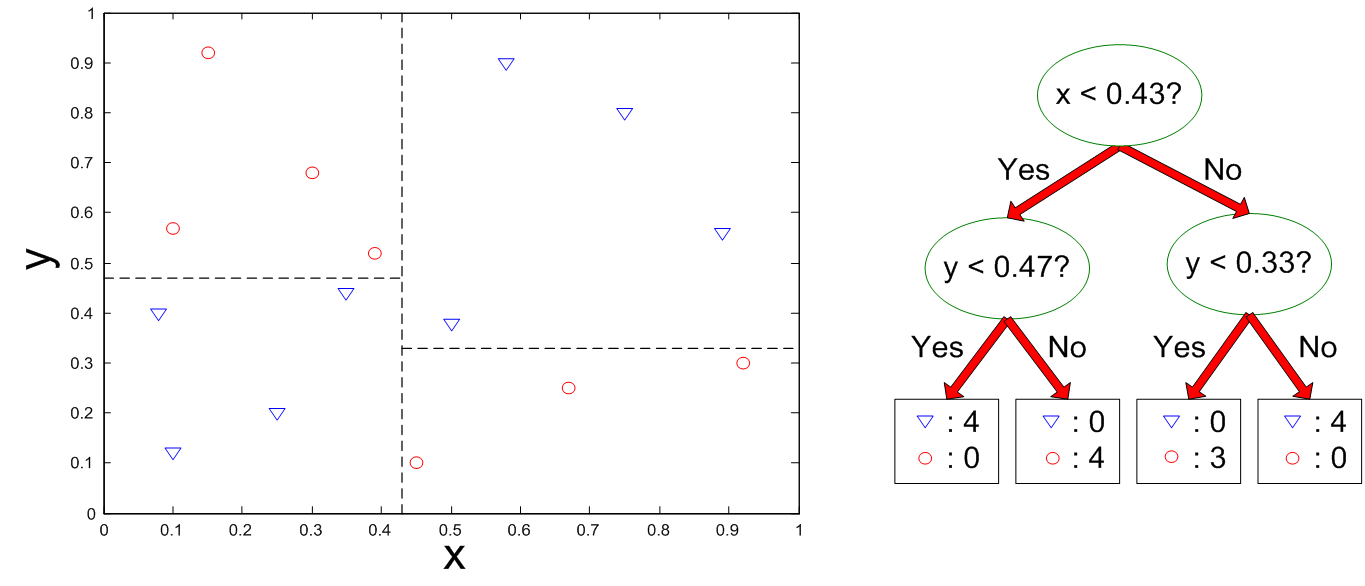
\includegraphics[width=0.8\linewidth,keepaspectratio]{decbound}
\end{center}
\begin{itemize}
	\item Border line between two neighboring regions of different classes is known as decision boundary
\item  Decision boundary is parallel to axes because test condition involves a single attribute at-a-time
	\end{itemize}
\end{frame}

%%%%%%%%%%%%%%%%%%%%%%%%%%%%%%%%%%%%%%%%%%%%%%%%%%%%%%%%%%
\begin{frame}[fragile]\frametitle{Decision Trees}
Simple, yet widely used classification technique 

\begin{itemize}
\item For categorical target variables. There also are Regression trees, for continuous target variables
\item Predictor Features: binary, nominal, ordinal, discrete, continuous.
\item Evaluating the model: One metric: error rate in predictions
\end{itemize}
\end{frame}

%%%%%%%%%%%%%%%%%%%%%%%%%%%%%%%%%%%%%%%%%%%%%%%%%%%%%%%%%%%%%%%%%%%%%%%%
\begin{frame}[fragile]\frametitle{Decision Trees Structure}
\begin{itemize}
			\item {\bf A root node} has no incoming edges and zero or more outgoing edges
			\item {\bf Internal nodes}, each of which has exactly one incoming edge and 
			two or more outgoing edges. An internal node is a new question.  
			\item{\bf Leaf/terminal nodes} , each of which has exactly one incoming edge
			and no outgoing edges. Is a class label. If a leaf node is reached, you got the
			conclusion. 
\end{itemize}
\end{frame}


%%%%%%%%%%%%%%%%%%%%%%%%%%%%%%%%%%%%%%%%%%%%%%%%%%%%%%%%%%%%%%%%%%%%%%%%
\begin{frame}[fragile]\frametitle{Decision Trees}
\begin{itemize}
			\item Were really popular 2 decades ago, but fail out of fashion due to over fitting
			\item Then came newer versions like C4.5, C5 to address some of the issues
			\item Rather than a single tree, it was found that collection of trees addresses this variance/over-fitting problem
			\item Thus, now we have Random Forest and Boosting, to make Trees as sought after solution.
\end{itemize}
\end{frame}

%%%%%%%%%%%%%%%%%%%%%%%%%%%%%%%%%%%%%%%%%%%%%%%%%%%%%%%%%%%%%%%%%%%%%%%%%%%%%%%%%%
\begin{frame}[fragile]\frametitle{}
\begin{center}
{\Large Decision Tree for Loan Default}
\end{center}
\end{frame}


%%%%%%%%%%%%%%%%%%%%%%%%%%%%%%%%%%%%%%%%%%%%%%%%%%%%%%%%%%
\begin{frame}[fragile]\frametitle{Decision Trees}
\begin{center}
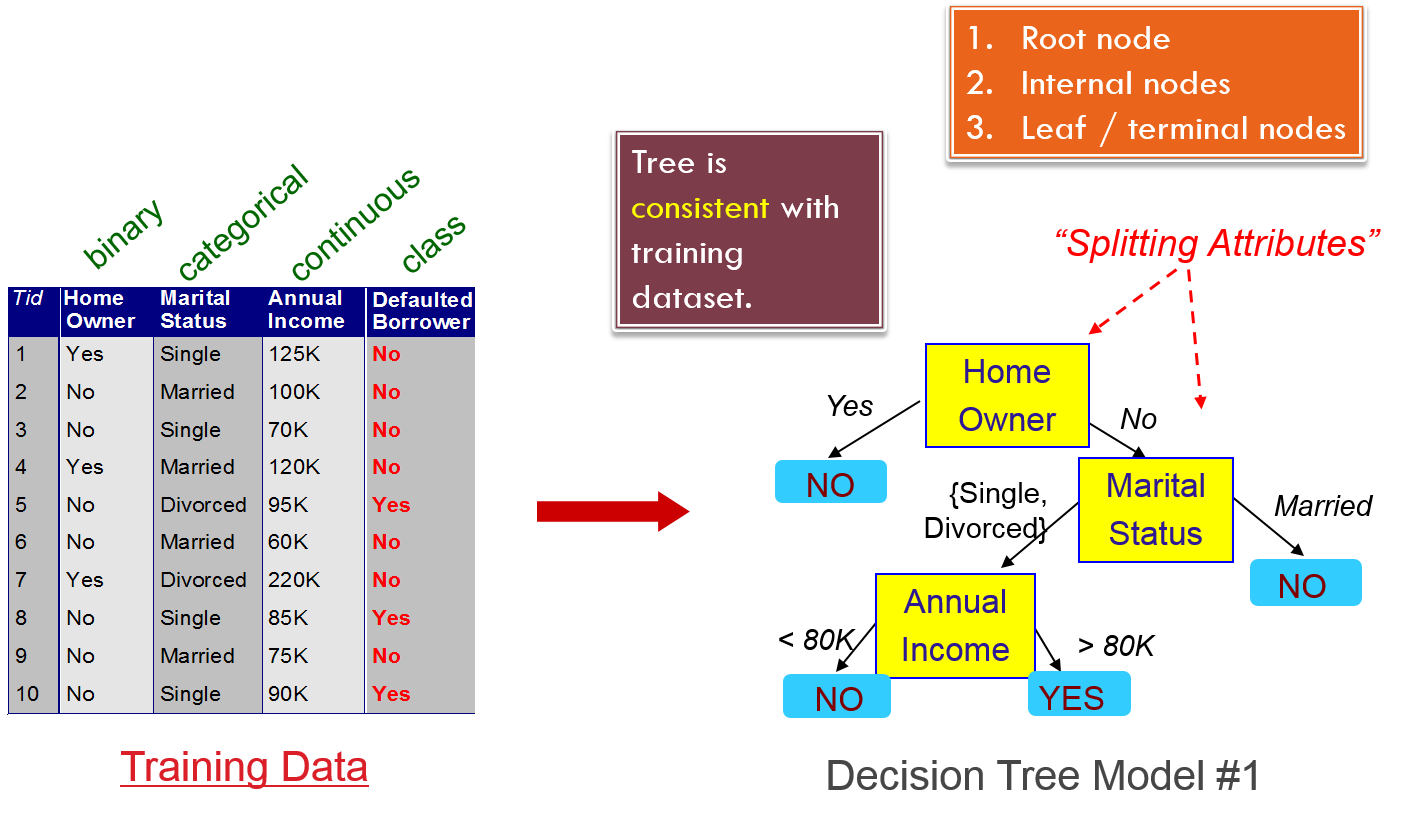
\includegraphics[width=\linewidth,keepaspectratio]{treesplit}
\end{center}
\end{frame}

%%%%%%%%%%%%%%%%%%%%%%%%%%%%%%%%%%%%%%%%%%%%%%%%%%%%%%%%%%
\begin{frame}[fragile]\frametitle{Decision Trees}
\begin{center}
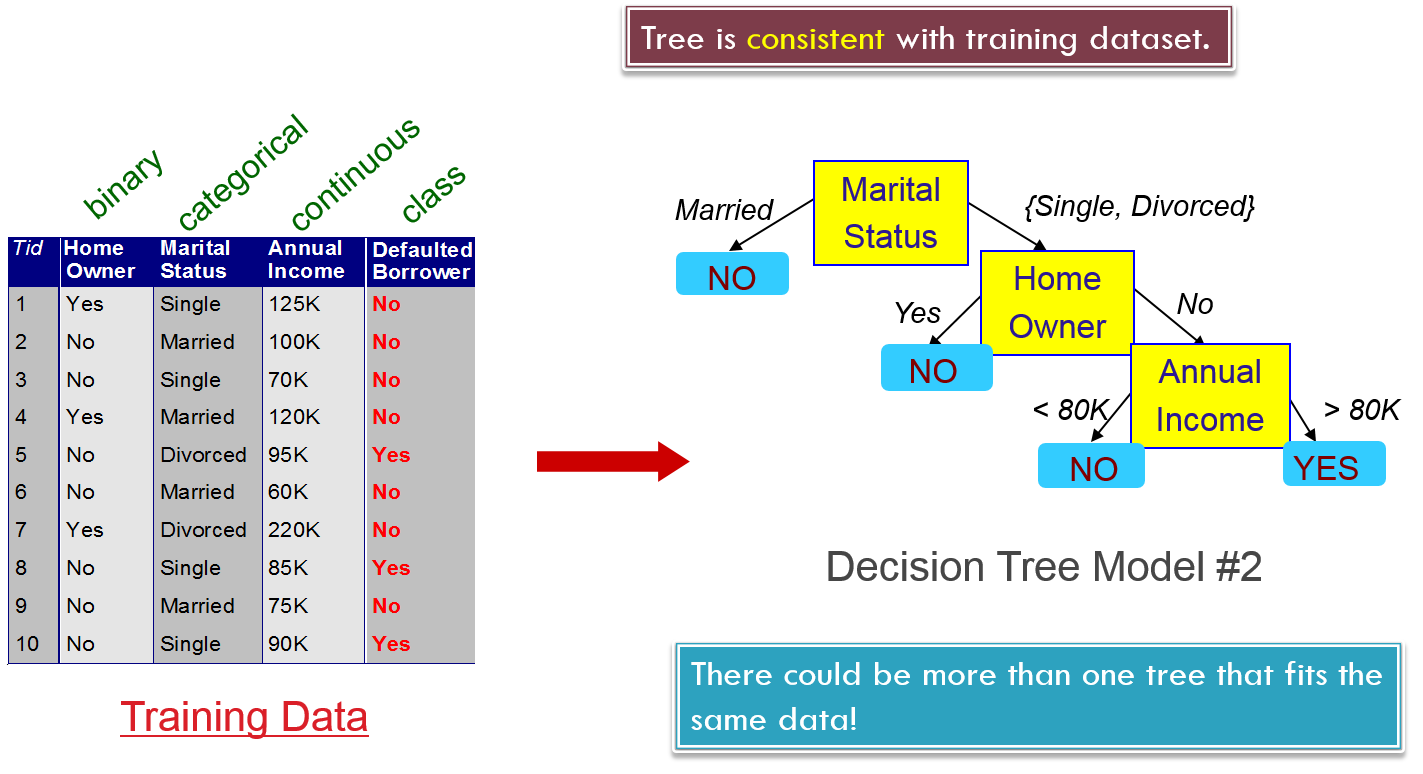
\includegraphics[width=\linewidth,keepaspectratio]{treesplit2}
\end{center}
\end{frame}

%%%%%%%%%%%%%%%%%%%%%%%%%%%%%%%%%%%%%%%%%%%%%%%%%%%%%%%%%%
\begin{frame}[fragile]\frametitle{Apply Model to Test Data}
\begin{center}
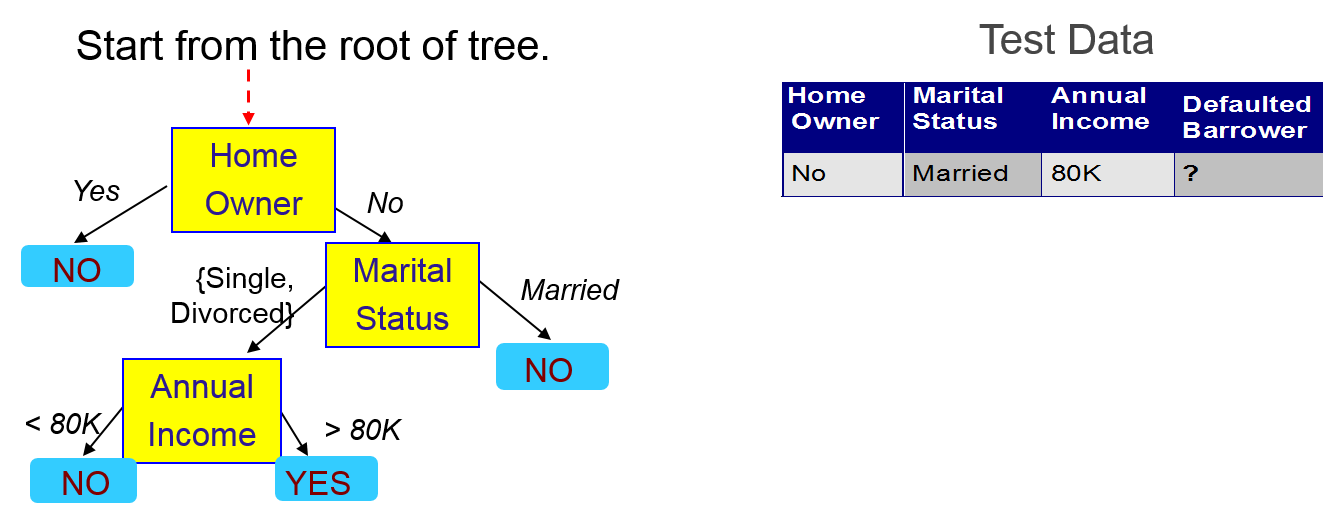
\includegraphics[width=\linewidth,keepaspectratio]{treetest}
\end{center}
\end{frame}

%%%%%%%%%%%%%%%%%%%%%%%%%%%%%%%%%%%%%%%%%%%%%%%%%%%%%%%%%%%%%%%%%%%%%%%%%%%%%%%%%%
\begin{frame}[fragile]\frametitle{}
\begin{center}
{\Large Decision Tree for 'Will John Play?'}
\end{center}
\end{frame}


%%%%%%%%%%%%%%%%%%%%%%%%%%%%%%%%%%%%%%%%%%%%%%%%%%%%%%%%%%
\begin{frame}[fragile]\frametitle{Predict if John will play tennis}

\begin{itemize}
\item We have records of outdoors condition and whether John played on those days or not. 
\item That's the training data.
\item We wish to predict for certain UNSEEN condition, whether John will play or not.
\end{itemize}
\begin{center}
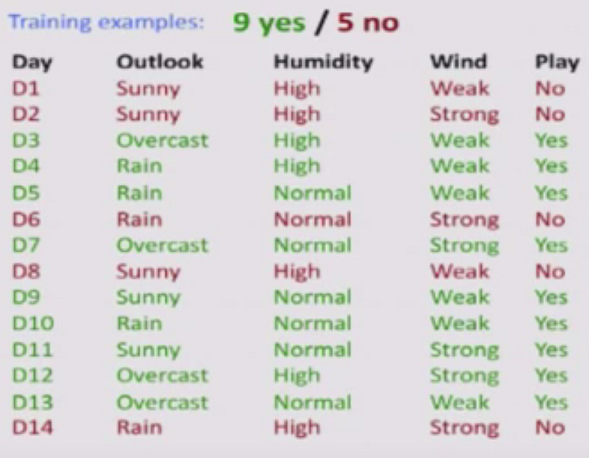
\includegraphics[width=0.5\linewidth,keepaspectratio]{dt1}
\end{center}
\tiny{(Ref: Decision Trees - Victor Lavrenko)}
\end{frame}

%%%%%%%%%%%%%%%%%%%%%%%%%%%%%%%%%%%%%%%%%%%%%%%%%%%%%%%%%%
\begin{frame}[fragile]\frametitle{Predict if John will play tennis}
Steps:
	\begin{itemize}
	\item Split at columns
 	\item Are	they pure? (all yes or all no)	
 	\item If yes: stop; if not: repeat
	\end{itemize}

Lets start with first column'' ``Outlook''
\end{frame}

%%%%%%%%%%%%%%%%%%%%%%%%%%%%%%%%%%%%%%%%%%%%%%%%%%%%%%%%%%
\begin{frame}[fragile]\frametitle{Predict if John will play tennis}
\begin{center}
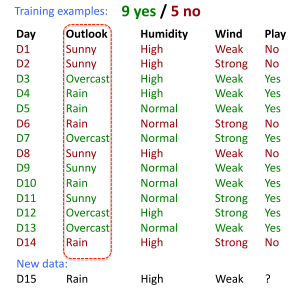
\includegraphics[width=0.5\linewidth,keepaspectratio]{dt2}
\end{center}
\end{frame}


%%%%%%%%%%%%%%%%%%%%%%%%%%%%%%%%%%%%%%%%%%%%%%%%%%%%%%%%%%
\begin{frame}[fragile]\frametitle{Predict if John will play tennis}
\begin{center}
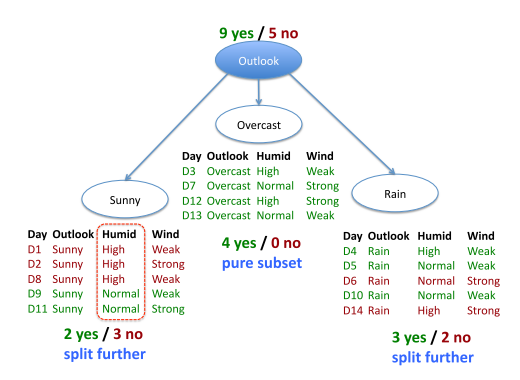
\includegraphics[width=0.6\linewidth,keepaspectratio]{dt3}
\end{center}
	\begin{itemize}
	\item Outlook-Overcast turned Pure , in the first split itself!!
	\item Humidity and Wind are irrelevant for this middle node now.
	\item Cannot expand this middle node further. 
	\item Go for the other nodes: Outlook-Sunny and Outlook-Rain
	\end{itemize}
\end{frame}

%%%%%%%%%%%%%%%%%%%%%%%%%%%%%%%%%%%%%%%%%%%%%%%%%%%%%%%%%%
\begin{frame}[fragile]\frametitle{Predict if John will play tennis}
\begin{center}
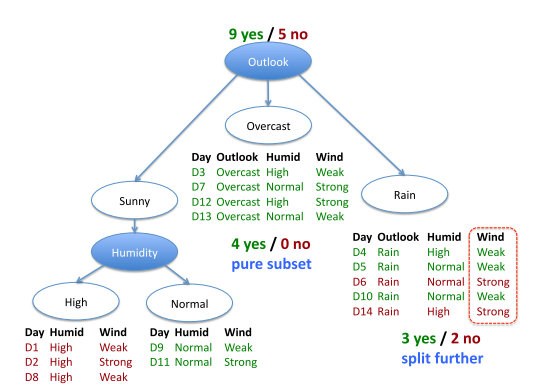
\includegraphics[width=0.5\linewidth,keepaspectratio]{dt4}
\end{center}
	\begin{itemize}
	\item Outlook-Sunny after splitting on Humidity turned Pure
	\item Need Outlook-Rain to split now.
	\end{itemize}

\end{frame}


%%%%%%%%%%%%%%%%%%%%%%%%%%%%%%%%%%%%%%%%%%%%%%%%%%%%%%%%%%
\begin{frame}[fragile]\frametitle{Predict if John will play tennis}

	\begin{itemize}
	\item Rain after splitting on Wind turned Pure.
	\item All leaves are Pure now.
	\item That's the end of splitting
	\end{itemize}
\begin{center}
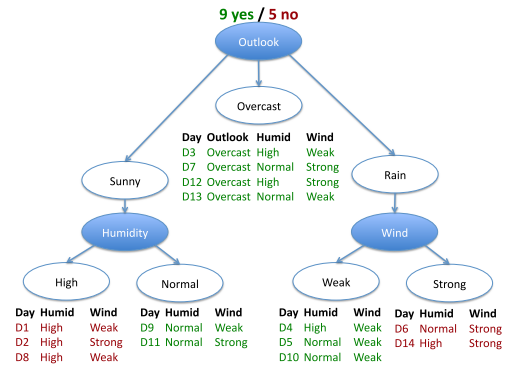
\includegraphics[width=0.5\linewidth,keepaspectratio]{dt5}
\end{center}
\end{frame}

%%%%%%%%%%%%%%%%%%%%%%%%%%%%%%%%%%%%%%%%%%%%%%%%%%%%%%%%%%
\begin{frame}[fragile]\frametitle{Predict if John will play tennis}

	\begin{itemize}
	\item Decision tree result can be seen below.
	\item To test the unseen condition, traverse the tree
	\item for Day 15, with Outlook-Rain, Humid-High and Wind-Weak, the outcome is ``Yes''.  John will play.
	\end{itemize}
\begin{center}
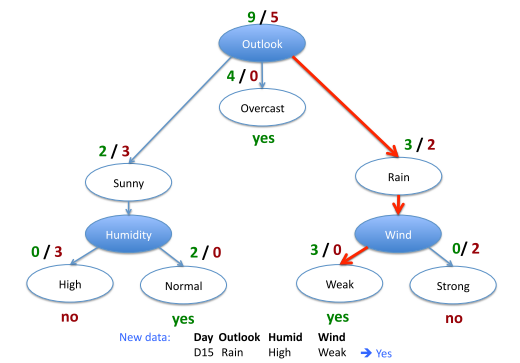
\includegraphics[width=0.6\linewidth,keepaspectratio]{dt6}
\end{center}
\end{frame}


%%%%%%%%%%%%%%%%%%%%%%%%%%%%%%%%%%%%%%%%%%%%%%%%%%%%%%%%%%
\begin{frame}[fragile]\frametitle{Decision Tree Classifier}
\begin{itemize}
\item Decision tree models are relatively more descriptive than other types of classifier models
\begin{itemize}
\item Easier interpretation
\item Easier to explain predicted values
\end{itemize}
\item Exponentially many decision trees can be built
\item Which is best? Some trees will be more accurate than others
\item How to construct the tree? Computationally infeasible to try every possible tree.
\end{itemize}
\end{frame}

%%%%%%%%%%%%%%%%%%%%%%%%%%%%%%%%%%%%%%%%%%%%%%%%%%%%%%%%%%
\begin{frame}[fragile]\frametitle{Decision Tree Inventor}
\begin{itemize}
\item The late Leo Breiman was instrumental in developing several tree-based methods. 
\item Worked on the problem of classifying ships from radar signals. 
\item He covered the walls of his office with data from the radars prior to his “aha” moment on Decision Trees.
\end{itemize}

\begin{center}
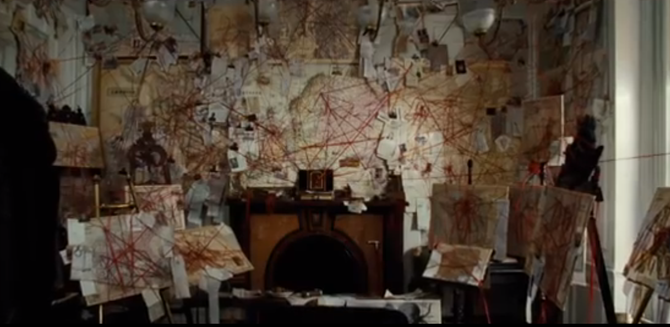
\includegraphics[width=0.6\linewidth,keepaspectratio]{dt25}

(Something like this!!!)
\end{center}

See: ``Leo Breiman (CART)'' video on Youtube
\end{frame}

%%%%%%%%%%%%%%%%%%%%%%%%%%%%%%%%%%%%%%%%%%%%%%%%%%%%%%%%%%%%%%%%%%%%%%%%%%%%%%%%%%
\begin{frame}[fragile]\frametitle{}
\begin{center}
{\Large Building the Decision Tree}
\end{center}
\end{frame}


%%%%%%%%%%%%%%%%%%%%%%%%%%%%%%%%%%%%%%%%%%%%%%%%%%%%%%%%%%
\begin{frame}[fragile]\frametitle{Formally}
\begin{itemize}
\item A decision tree has three types of nodes:

\begin{itemize}
\item A root node that has no incoming edges and zero or mode outgoing edges
\item Internal nodes, each of which has exactly one incoming edge and two or more outgoing edges
\item Leaf nodes (or terminal nodes), each of which has exactly one incoming edge and no outgoing edges
\end{itemize}
\item Each leaf node is assigned a class label
\item Non-terminal nodes contain attribute test conditions to separate records that have different characteristics
\end{itemize}
\end{frame}

%%%%%%%%%%%%%%%%%%%%%%%%%%%%%%%%%%%%%%%%%%%%%%%%%%%%%%%%%%
\begin{frame}[fragile]\frametitle{What is the ``Best Attribute'' to split}
There are different criteria that can be used to determine what 
is the best attribute to split.
\begin{itemize}
\item Information Gain
\item Gini Index
\item \ldots
% \item Classification Error
% \item Gain Ratio (Normalized Information Gain)
% \item Variance Reduction
\end{itemize}
\end{frame}

%%%%%%%%%%%%%%%%%%%%%%%%%%%%%%%%%%%%%%%%%%%%%%%%%%%%%%%%%%
\begin{frame}[fragile]\frametitle{Which attribute to split on}

	\begin{itemize}
	\item Want to measure PURITY of the split
	\item Are we more certain about Yes/No after the split?
		\begin{itemize}
		\item pure set (4 yes/ 0 no) then completely certain (100\%)
		\item impure set (3 yes/ 3 no) then completely uncertain (50\%)
		\end{itemize}
	\item Must be symmetric: 4 yes / 0 no as pure s 0 yes/ 4 no.
	\end{itemize}
\begin{center}
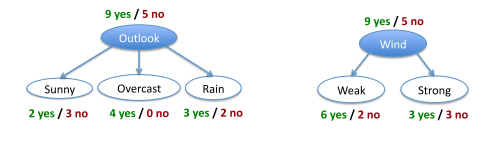
\includegraphics[width=0.8\linewidth,keepaspectratio]{dt7}
\end{center}
\end{frame}

%%%%%%%%%%%%%%%%%%%%%%%%%%%%%%%%%%%%%%%%%%%%%%%%%%%%%%%%%%
\begin{frame}[fragile]\frametitle{Entropy}
\begin{itemize}
\item High `mixed'-ness, high uncertainty thus higher ``entropy''
\item Say if  all are identical members, then no uncertainty and thus zero ``entropy''.
\end{itemize}
\end{frame}

%%%%%%%%%%%%%%%%%%%%%%%%%%%%%%%%%%%%%%%%%%%%%%%%%%%%%%%%%%
\begin{frame}[fragile]\frametitle{Entropy}
\begin{itemize}
\item So, when we split a set we want the halves to be more distinct from each other and the members in the group to be more like each other
\item We want entropy to go down as we keep splitting.
\item So if we use an approach/split that doesn't reduce the entropy by much, then it is probably not a good attribute or a good value to split on.
\item Shannon's entropy is defined for a system with N possible states as 
$\Large S = -\sum_{i=1}^{N}p_i \log_2{p_i}$  where $p_i$  is the probability of finding the system in the  $i$-th state.
\item $N$ designates number of classes. For binary classification $N=2$.
\item Shannon's formula is part of information theory, given minimum number of letters to encode a message.
\end{itemize}
\end{frame}

%%%%%%%%%%%%%%%%%%%%%%%%%%%%%%%%%%%%%%%%%%%%%%%%%%%%%%%%%%
\begin{frame}[fragile]\frametitle{Entropy}
\begin{itemize}
\item Originally from Second Law of Thermodynamics, Entropy is a measure of disorder (uncertainty, chaos).
\item In the current context, its measure of disorder in the target-label.
\item  Entropy can be described as the degree of chaos in the system.
\item The higher the entropy, the less ordered the system and vice versa.
\item Information Gain is a measure of decrease in Entropy by partitioning the data-set.
\end{itemize}
\end{frame}

%%%%%%%%%%%%%%%%%%%%%%%%%%%%%%%%%%%%%%%%%%%%%%%%%%%%%%%%%%
\begin{frame}[fragile]\frametitle{How to determine the Best Split?}
How does entropy help us?

\begin{center}
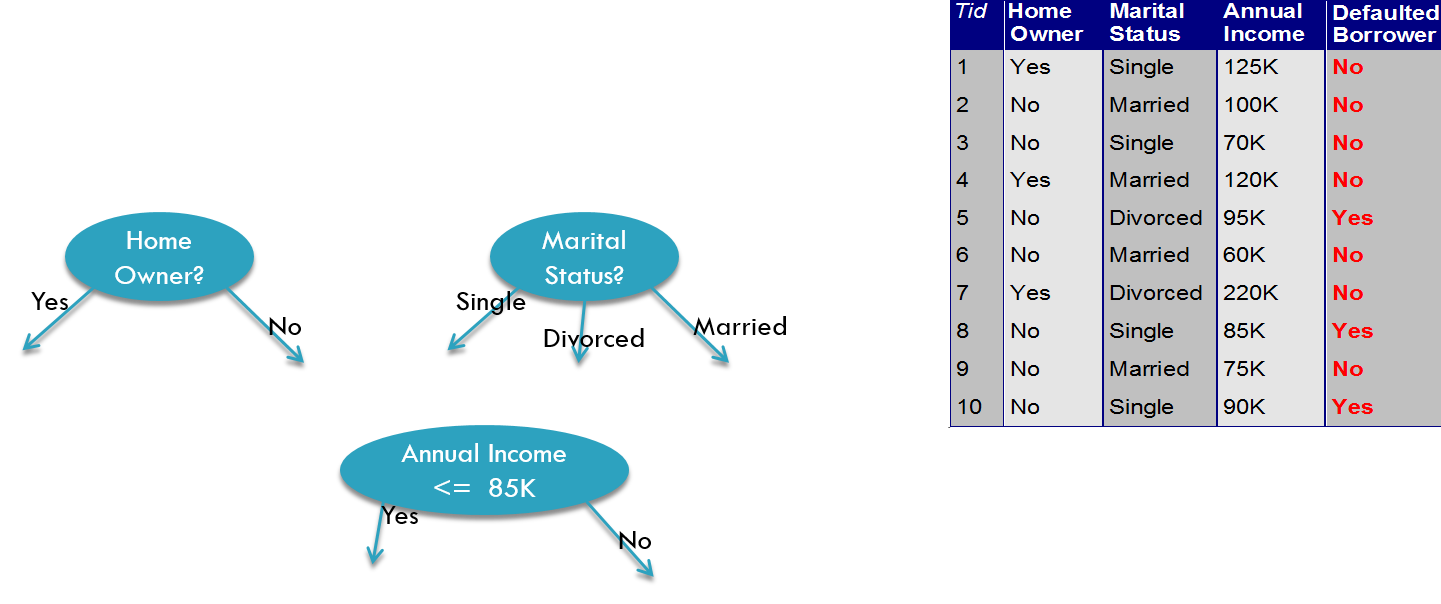
\includegraphics[width=\linewidth,keepaspectratio]{splitent}
\end{center}
\end{frame}


%%%%%%%%%%%%%%%%%%%%%%%%%%%%%%%%%%%%%%%%%%%%%%%%%%%%%%%%%%%%%%%%%%%%%%%%%%%%%%%%%%
\begin{frame}[fragile]\frametitle{}
\begin{center}
{\Large How to calculate Information Gain using Entropy?}
\end{center}
\end{frame}

%%%%%%%%%%%%%%%%%%%%%%%%%%%%%%%%%%%%%%%%%%%%%%%%%%%%%%%%%%
\begin{frame}[fragile]\frametitle{Information Gain}
\begin{itemize}
\item Want many items in pure sets.
\item Try to split on each possible feature in a dataset. See which split works ``best''.
\item Measure the reduction in the overall entropy of a set of instances.
\end{itemize}
$InformationGain = Entropy(s) - \sum \frac{s_i}{s} E(s_i)$
\end{frame}


%%%%%%%%%%%%%%%%%%%%%%%%%%%%%%%%%%%%%%%%%%%%%%%%%%%%%%%%%%
\begin{frame}[fragile]\frametitle{Entropy}
\begin{itemize}
\item ID3 algorithm uses entropy to calculate the homogeneity of a sample. 
\item If the sample is completely homogeneous the entropy is zero 
\item If the sample is equally divided then it has entropy of one.
\item By Binary outcome, $Entropy(n) = - p_{(+)} log_2 p_{(+)} - p_{(-)} log_2 p_{(-)}$
\item $Entropy(n) = - 0.5 log_2 0.5 - 0.5 log_2 0.5 = 1$
\end{itemize}
\begin{center}
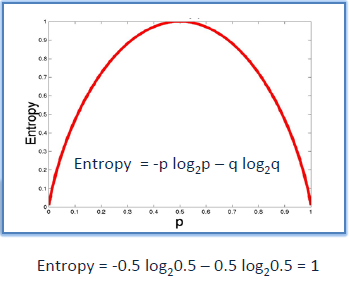
\includegraphics[width=0.4\linewidth,keepaspectratio]{dt11}
\end{center}
\end{frame}


%%%%%%%%%%%%%%%%%%%%%%%%%%%%%%%%%%%%%%%%%%%%%%%%%%%%%%%%%%
\begin{frame}[fragile]\frametitle{Entropy}
In our original example:
\begin{itemize}
% \item Being Binary, Play or No-Play, $Entropy(n) = - p_{(+)} log_2 p_{(+)} - p_{(-)} log_2 p_{(-)}$
% \item Sum of \% of positive/negative examples in $X$
\item Impure ( 3 yes/ 3 no): $Entropy(n) = - 3/6  log_2 3/6 - 3/6 log_2 3/6 = 1$
\item Pure ( 4 yes/ 0 no): $Entropy(n) = - 4/4  log_2 4/4 - 0/4 log_2 0/4 = 0$
\item So, Entropy also ranges from 0 to 1, in following fashion
\end{itemize}
\begin{center}
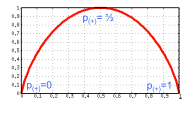
\includegraphics[width=0.5\linewidth,keepaspectratio]{dt8}
\end{center}
\end{frame}

%%%%%%%%%%%%%%%%%%%%%%%%%%%%%%%%%%%%%%%%%%%%%%%%%%%%%%%%%%
\begin{frame}[fragile]\frametitle{Entropy}
\begin{itemize}

\item $Entropy(n) = - \sum_i^c p_i log_2 p_i$
\item Weighted sum of the logs of the probabilities of each of the possible outcomes
\item Entropy of the set of 52 playing cards: Randomly selecting any specific card i is 1/52. $Entropy(n) = - \sum_1^{52} 0.019 log_2 0.019 = 5.7$
\item Entropy of the set of 4 suits: Randomly selecting any specific card i is 1/4. $Entropy(n) = - \sum_1^{4} 0.25 log_2 0.25 = 2$
\item The higher the impurity, the higher the entropy.
\item That's the Reason for Using the log function
\end{itemize}
\end{frame}

% %%%%%%%%%%%%%%%%%%%%%%%%%%%%%%%%%%%%%%%%%%%%%%%%%%%%%%%%%%
% \begin{frame}[fragile]\frametitle{Entropy}
% \begin{center}
% 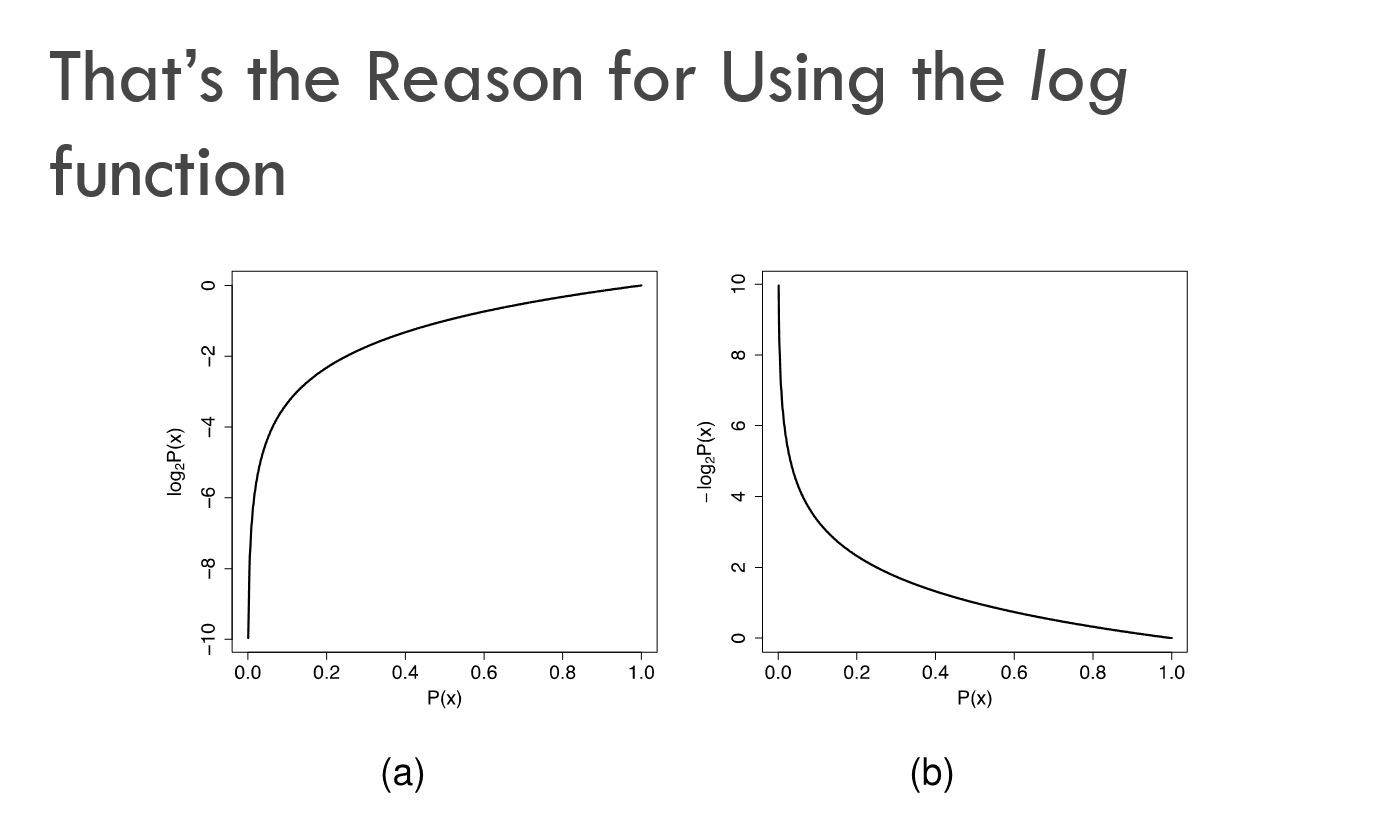
\includegraphics[width=\linewidth,keepaspectratio]{logent}
% \end{center}
% \end{frame}


% %%%%%%%%%%%%%%%%%%%%%%%%%%%%%%%%%%%%%%%%%%%%%%%%%%%%%%%%%%%%%%%%%%%%%%%%%%%%%%%%%%
% \begin{frame}[fragile]\frametitle{}
% \begin{center}
% {\Large Toy Example}
% \end{center}
% \end{frame}

% %%%%%%%%%%%%%%%%%%%%%%%%%%%%%%%%%%%%%%%%%%%%%%%%%%%%%%%%%%
% \begin{frame}[fragile]\frametitle{Splitting across Category (no threshold)}
% \begin{itemize}
% \item Say if you are working on predicting political liking of a person.
% \item Labels could be political parties like BJP, Congress, NCP, etc.
% \item Each of these parties will have certain number of followers.
% \item $p_i$ is say probability of being followed by $i$th party.
% \item Say, if BJP is being followed by 60 people, its $p_1=60/100 =0.6$, similarly for others.

% \end{itemize}
% \begin{center}
% 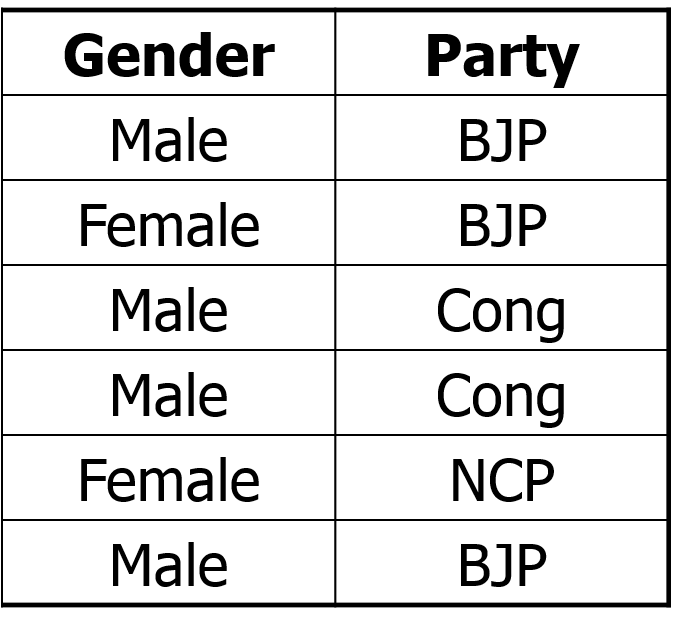
\includegraphics[width=0.35\linewidth,keepaspectratio]{splitbjp}
% \end{center}
% \end{frame}

% %%%%%%%%%%%%%%%%%%%%%%%%%%%%%%%%%%%%%%%%%%%%%%%%%%%%%%%%%%
% \begin{frame}[fragile]\frametitle{Entropy of only the resultant column, baseline}
% \begin{itemize}
% \item Entropy for vector $d$ is given by $E(\bar{d}) = -\sum p_i log(p_i)$
% \item log of probability (between 0 to 1) is negative, so to make Entropy as a positive value,  -ve is put.
% \item $E(\bar{d}) = - (p_{bjp} log(p_{bjp}) + p_{con} log(p_{con}) + p_{ncp} log(p_{ncp})) $
% \item $E(\bar{d}) = - (0.6 log(0.6) + 0.3 log(0.3) + 0.1 log(0.1)) $
% \end{itemize}
% Small note, assume: $0log0 = 0$
% \end{frame}

% %%%%%%%%%%%%%%%%%%%%%%%%%%%%%%%%%%%%%%%%%%%%%%%%%%%%%%%%%%
% \begin{frame}[fragile]\frametitle{Entropy after Partition by an attribute}
% \begin{itemize}
% \item Entropy of a Partition is  sum of weighted average of Entropies of each partition
% \item Here, if we partition based on Male Female. Then weights would be probability of being Male or Female.
% \item  $E(\bar{d},\bar{a}) = \sum (\frac{n_j}{n} \times E(\bar{d}_j)))$
% \item  Men and Women are tracked in the other vector $\bar{a}$
% \item So probability after partition is : Entropy for Men times probability of picking a man, plus, Entropy for women times probability of picking a woman
% \end{itemize}
% \end{frame}


% %%%%%%%%%%%%%%%%%%%%%%%%%%%%%%%%%%%%%%%%%%%%%%%%%%%%%%%%%%
% \begin{frame}[fragile]\frametitle{Information Gain}
% \begin{itemize}
% \item Information Gain due to partition due to $\bar{a}$ is given by: $I(\bar{d},\bar{a}) = E(\bar{d},\bar{a}) - E(\bar{d}) $
% \item So, split with the column where Information Gain is Max.
% \end{itemize}
% \end{frame}

% %%%%%%%%%%%%%%%%%%%%%%%%%%%%%%%%%%%%%%%%%%%%%%%%%%%%%%%%%%
% \begin{frame}[fragile]\frametitle{Toy Example, Splitting across number (threshold)}
% We will predict the color of the ball based on its position.
% \begin{center}
% 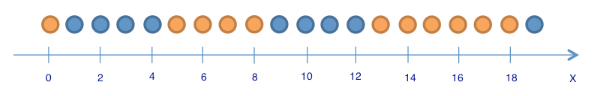
\includegraphics[width=0.8\linewidth,keepaspectratio]{dttoy1}
% \end{center}

% There are 9 blue balls and 11 yellow balls.


% {\tiny (Ref: MLCourse.ai - Decision Tree https://www.kaggle.com/kashnitsky/topic-3-decision-trees-and-knn )}
% \end{frame}

% %%%%%%%%%%%%%%%%%%%%%%%%%%%%%%%%%%%%%%%%%%%%%%%%%%%%%%%%%%
% \begin{frame}[fragile]\frametitle{Toy Example, Splitting across number (threshold)}
% \begin{itemize}
% \item If we randomly pull out a ball, then it will be blue with probability  $p_1=\frac{9}{20}$ and yellow with probability $p_2=\frac{11}{20}$
% \item Mixed-ness is given by the entropy $S_0 = -\frac{9}{20}\log_2{\frac{9}{20}}-\frac{11}{20}\log_2{\frac{11}{20}} \approx 1$
% \item Why it is so close to 1? 
% \end{itemize}
% \end{frame}

% %%%%%%%%%%%%%%%%%%%%%%%%%%%%%%%%%%%%%%%%%%%%%%%%%%%%%%%%%%
% \begin{frame}[fragile]\frametitle{Toy Example, Splitting across number (threshold)}
% \begin{itemize}
% \item As there are almost equal number of blue and yellow balls and if we pick random one, we are not going to know what it will be. So entropy is Max.
% \item This value by itself may not tell us much, but let's see how the value changes if we were to break the balls into two groups: with the position less than or equal to 12 and greater than 12.
% \item Say, in case both groups have exact same numbers then $P_1 = P_2 = 0.5$.
% \item Entropy would be $S_0 = -\frac{1}{2}\log_2{\frac{1}{2}}-\frac{1}{2}\log_2{\frac{1}{2}}$
% \item As we know $log_2{\frac{1}{2}} = -1$ (Note: $2^{-1} = \frac{1}{2}$), the total entropy is 1.
% \end{itemize}
% \end{frame}

% %%%%%%%%%%%%%%%%%%%%%%%%%%%%%%%%%%%%%%%%%%%%%%%%%%%%%%%%%%
% \begin{frame}[fragile]\frametitle{Toy Example, Splitting across number (threshold)}
% \begin{center}
% 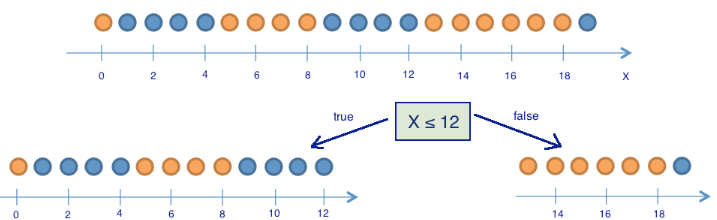
\includegraphics[width=0.8\linewidth,keepaspectratio]{dttoy2}
% \end{center}

% \begin{itemize}
% \item The left group has 13 balls, 8 blue and 5 yellow. The entropy of this group is $S_1 = -\frac{5}{13}\log_2{\frac{5}{13}}-\frac{8}{13}\log_2{\frac{8}{13}} \approx 0.96$
% \item he right group has 7 balls, 1 blue and 6 yellow. The entropy of the right group is  $S_2 = -\frac{1}{7}\log_2{\frac{1}{7}}-\frac{6}{7}\log_2{\frac{6}{7}} \approx 0.6$
% \end{itemize}

% \end{frame}

% %%%%%%%%%%%%%%%%%%%%%%%%%%%%%%%%%%%%%%%%%%%%%%%%%%%%%%%%%%
% \begin{frame}[fragile]\frametitle{Toy Example, Splitting across number (threshold)}
% \begin{itemize}
% \item Entropy has decreased in both groups, more so in the right group. 
% \item Since entropy is, in fact, the degree of chaos (or uncertainty) in the system, the reduction in entropy, as saw before, is called information gain. 
% \item Here, as we are splitting based on variable $Q$ (which is $x \leq 12$ is defined as $\Large IG(Q) = S_O - \sum_{i=1}^{q}\frac{N_i}{N}S_i,$, where  $q$  is the number of groups after the split,  
% $N_i$  is number of objects from the sample in which variable  $Q$  is equal to the  $i$-th value. 
% \end{itemize}
% \end{frame}

% %%%%%%%%%%%%%%%%%%%%%%%%%%%%%%%%%%%%%%%%%%%%%%%%%%%%%%%%%
% \begin{frame}[fragile]\frametitle{Toy Example, Splitting across number (threshold)}
% \begin{itemize}
% \item In our example, our split yielded two groups ( $q=2$ ), one with 13 elements ( $N_1=13$ ), the other with 7 ( $N_2=7$ ). Therefore, we can compute the information gain as $\Large IG(x \leq 12) = S_0 - \frac{13}{20}S_1 - \frac{7}{20}S_2 \approx 0.16.$
% \item It turns out that dividing the balls into two groups by splitting on ``coordinate is less than or equal to 12'' gave us a more ordered system.
% \item Let's continue to divide them into groups until the balls in each group are all of the same color.
% \end{itemize}
% \end{frame}

% %%%%%%%%%%%%%%%%%%%%%%%%%%%%%%%%%%%%%%%%%%%%%%%%%%%%%%%%%%
% \begin{frame}[fragile]\frametitle{Toy Example, Splitting across number (threshold)}
% \begin{center}
% 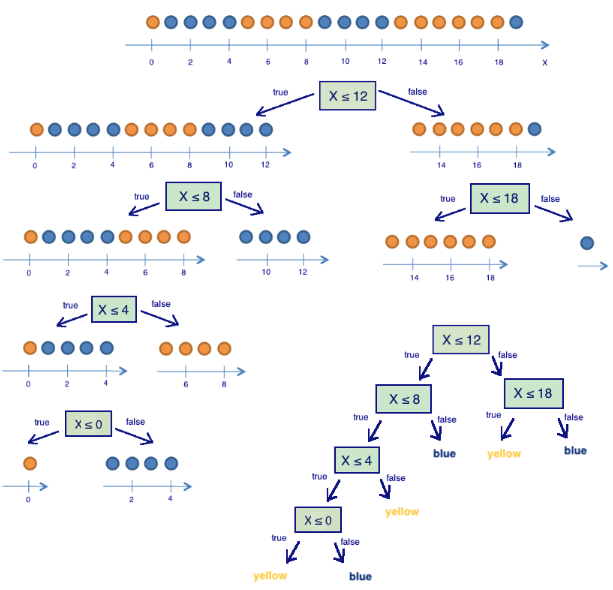
\includegraphics[width=0.6\linewidth,keepaspectratio]{dttoy3}
% \end{center}
% \end{frame}

% %%%%%%%%%%%%%%%%%%%%%%%%%%%%%%%%%%%%%%%%%%%%%%%%%%%%%%%%%
% \begin{frame}[fragile]\frametitle{Toy Example, Splitting across number (threshold)}
% \begin{itemize}
% \item For the right group, we can easily see that we only need one extra partition using ``coordinate less than or equal to 18''. 
% \item But, for the left group, we need three more. Note that the entropy of a group where all of the balls are the same color is equal to 0 ( $\log_2{1} = 0$ ).
% \item We have successfully constructed a decision tree that predicts ball color based on its position. This decision tree may not work well if we add any balls because it has perfectly fit to the training set (initial 20 balls). 
% \item If we wanted to do well in that case, a tree with fewer ``questions'' or splits would be more accurate, even if it does not perfectly fit the training set.
% \end{itemize}
% \end{frame}


%%%%%%%%%%%%%%%%%%%%%%%%%%%%%%%%%%%%%%%%%%%%%%%%%%%%%%%%%%%%%%%%%%%%%%%%%%%%%%%%%%
\begin{frame}[fragile]\frametitle{}
\begin{center}
{\Large Information Gain Exercise of Stars/Diamonds, Blue/Orange}
\end{center}
\end{frame}


%%%%%%%%%%%%%%%%%%%%%%%%%%%%%%%%%%%%%%%%%%%%%%%%%%%%%%%%%%
\begin{frame}[fragile]\frametitle{Entropy Example}
\begin{center}
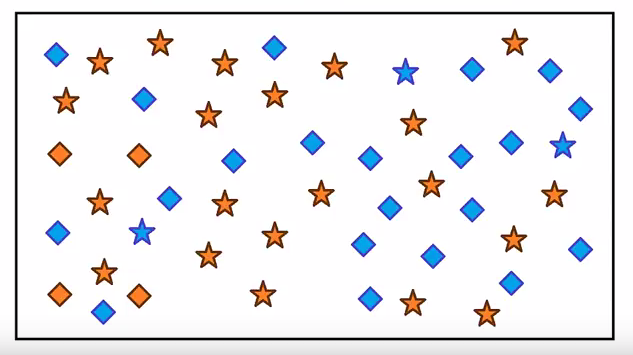
\includegraphics[width=0.6\linewidth,keepaspectratio]{stsq1}
\end{center}
\begin{itemize}
\item There are stars and diamonds, 24 stars, 25 diamonds
\item Input: Color
\item Output: Shape
%\item Partition these into boxes such that if I predict the type of object I will get.
%\item There is color also, so there are orange diamonds and blue diamonds. There are orange stars and blue stars.
\end{itemize}
\end{frame}


%%%%%%%%%%%%%%%%%%%%%%%%%%%%%%%%%%%%%%%%%%%%%%%%%%%%%%%%%%
\begin{frame}[fragile]\frametitle{Entropy Example}

\begin{itemize}
\item Predicting: Star vs Diamond
\item Split on: Color
\item Orange box and blue box.
\item With this, HAS it becomes easier to predict Star or Diamond?
\item Lesser chance of mis-classification. 
\item Less disorder, more information gain.
\end{itemize}
\begin{center}
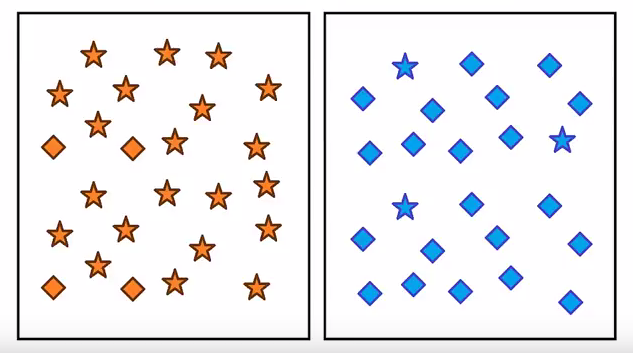
\includegraphics[width=0.6\linewidth,keepaspectratio]{stsq2}
\end{center}
\end{frame}


%%%%%%%%%%%%%%%%%%%%%%%%%%%%%%%%%%%%%%%%%%%%%%%%%%%%%%%%%%
\begin{frame}[fragile]\frametitle{Entropy Example}

\begin{itemize}
\item Full group : 24 stars, 25 diamonds
\item 25 orange object: 21 stars, 4 diamonds
\item 24 blue object: 3 stars, 21 diamonds
\item $p_{stars} = 24/49$ and  $p_{diamonds} = 25/49$ 
\end{itemize}
\begin{center}
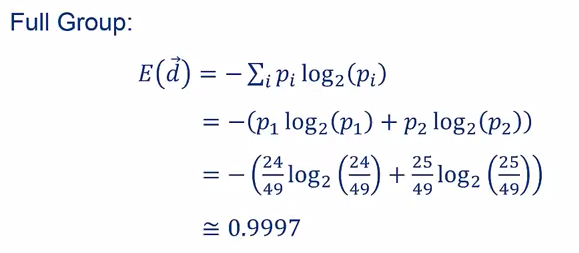
\includegraphics[width=0.6\linewidth,keepaspectratio]{stsq3}
\end{center}
This is Full Group, Original Entropy. Need to reduce it by partitioning.
\end{frame}

%%%%%%%%%%%%%%%%%%%%%%%%%%%%%%%%%%%%%%%%%%%%%%%%%%%%%%%%%%
\begin{frame}[fragile]\frametitle{Entropy Example}

\begin{itemize}
\item $p_{diamonds, orange} = 4/25$ and  $p_{stars,orange} = 21/25$ 
\item $p_{diamonds, blue} = 21/24$ and  $p_{stars,blue} = 3/24$ 
\end{itemize}

\begin{center}
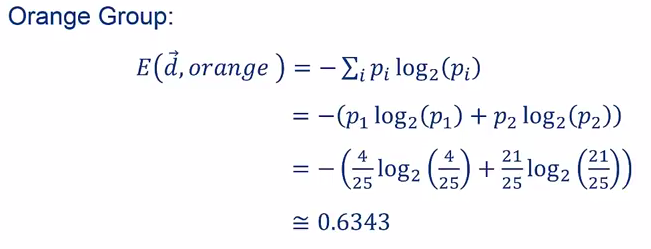
\includegraphics[width=0.6\linewidth,keepaspectratio]{stsq4} 

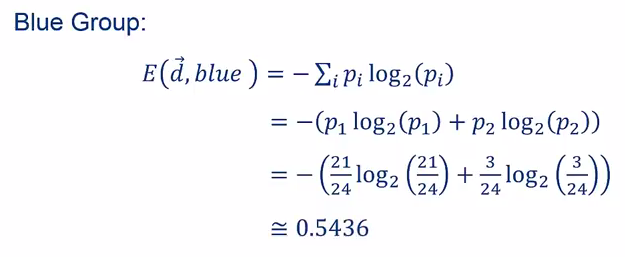
\includegraphics[width=0.6\linewidth,keepaspectratio]{stsq5}
\end{center}
\end{frame}

%%%%%%%%%%%%%%%%%%%%%%%%%%%%%%%%%%%%%%%%%%%%%%%%%%%%%%%%%%
\begin{frame}[fragile]\frametitle{Entropy Example}
\begin{itemize}
\item Original Full Group Entropy (without partitioning) was : 0.9997
\item Weighted sum after partitioning on Color
\end{itemize}
\begin{center}
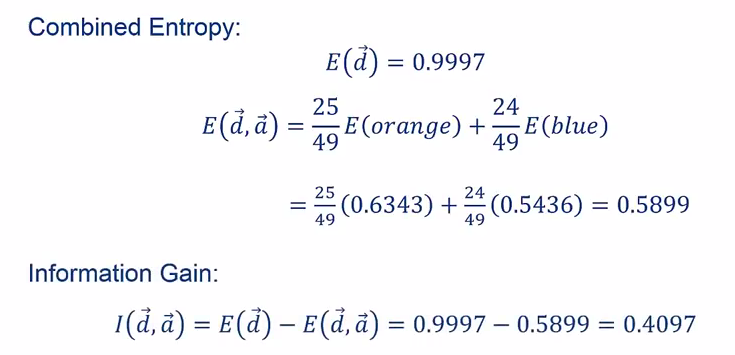
\includegraphics[width=0.6\linewidth,keepaspectratio]{stsq6}
\end{center}
Substantial gain.
\end{frame}


% %%%%%%%%%%%%%%%%%%%%%%%%%%%%%%%%%%%%%%%%%%%%%%%%%%%%%%%%%%%%%%%%%%%%%%%%%%%%%%%%%%
% \begin{frame}[fragile]\frametitle{}
% \begin{center}
% {\Large Tree Building Algorithm}
% \end{center}
% \end{frame}


% %%%%%%%%%%%%%%%%%%%%%%%%%%%%%%%%%%%%%%%%%%%%%%%%%%%%%%%%%%
% \begin{frame}[fragile]\frametitle{How to Build a Decision Tree?}
% \begin{itemize}
% \item Referred to as decision tree induction.
% \item Exponentially many decision trees can be constructed from a given set of attributes
% \item Infeasible to try them all to find the optimal tree
% \item Different ``decision tree building'' algorithms:
% \item CART, ID3, C4.5
% % \item Usually a greedy strategy is employed
% \end{itemize}
% \end{frame}


% %%%%%%%%%%%%%%%%%%%%%%%%%%%%%%%%%%%%%%%%%%%%%%%%%%%%
% %\begin{frame}[fragile]\frametitle{Hunt's Algorithm}
% % Recursive Procedure, where $D_t$ = set of training records that reach a node $t$. At Any node, 3 possibilities exist:
% %%\adjustbox{valign=t}{
% %%\begin{minipage}{0.45\linewidth}
% %\begin{itemize}
% %\item If all records in  $D_t$ belong to the same class, then  $t$ is a leaf node with class  $y_t$
% %\item If  $D_t$ is an empty set: then $t$t is a leaf node, class determined by the majority class of records in  $D_t$'s parent
% %\item If  $D_t$ contains records that belong to more than one class: use an attribute test to split the data into smaller subsets. Recursively apply the procedure to each subset.
% %\end{itemize}
% %%
% %%\end{minipage}
% %%}
% %%\hfill
% %%\adjustbox{valign=t}{
% %%\begin{minipage}{0.45\linewidth}
% %%\begin{center}
% %%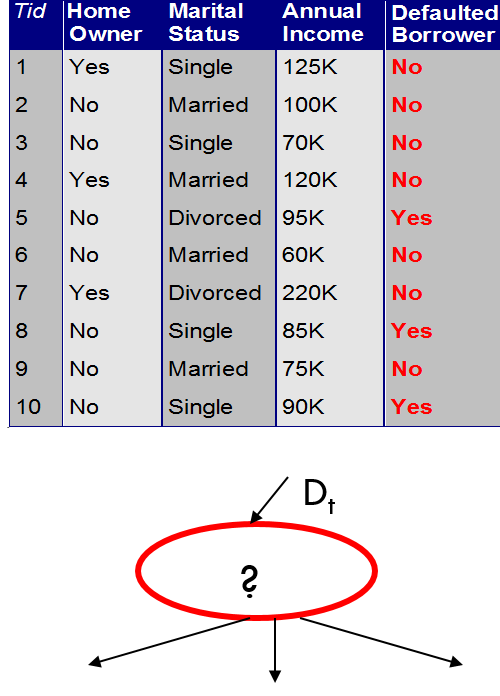
\includegraphics[width=\linewidth,keepaspectratio]{hunt1}
% %%\end{center}
% %%\end{minipage}
% %%}
% %\end{frame}
% %
% %%%%%%%%%%%%%%%%%%%%%%%%%%%%%%%%%%%%%%%%%%%%%%%%%%%%
% %\begin{frame}[fragile]\frametitle{Hunt's Algorithm}
% %
% %\adjustbox{valign=t}{
% %\begin{minipage}{0.45\linewidth}
% %\begin{itemize}
% %\item Tree begins with single node whose label reflects the majority class value
% %\item Tree needs to be refined because root node contains records from both classes
% %\item Divide records recursively into smaller subsets
% %
% %\end{itemize}
% %
% %\end{minipage}
% %}
% %\hfill
% %\adjustbox{valign=t}{
% %\begin{minipage}{0.45\linewidth}
% %\begin{center}
% %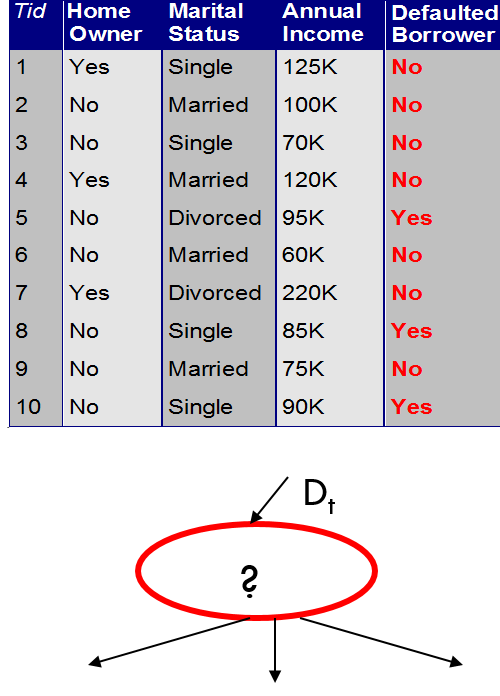
\includegraphics[width=\linewidth,keepaspectratio]{hunt1}
% %\end{center}
% %\end{minipage}
% %}
% %\end{frame}
% %
% %%%%%%%%%%%%%%%%%%%%%%%%%%%%%%%%%%%%%%%%%%%%%%%%%%%%%%%%%%%
% %\begin{frame}[fragile]\frametitle{Hunt's Algorithm}
% %\begin{itemize}
% %\item Hunt's Algorithm will work if:
% %\item Every combination of attribute values is present 
% %\begin{itemize}
% %\item Question: realistic or unrealistic?
% %\item Unrealistic: at least 2n records necessary for binary attributes
% %\item Examples: no record for {HomeOwner=Yes, Marrital=Single, Income=60K}
% %\item Each combination of attribute values has unique class label
% %\end{itemize}
% %\begin{itemize}
% %\item Question: realistic or unrealistic?
% %\item Unrealistic.
% %\item Example: Suppose we have two individuals, each with the properties {HomeOwner=Yes, Marrital=Single, Income=125K}, but one person defaulted and the other did not.
% %\end{itemize}
% %\end{itemize}
% %\end{frame}
% %
% %
% %%%%%%%%%%%%%%%%%%%%%%%%%%%%%%%%%%%%%%%%%%%%%%%%%%%%%%%%%%%
% %\begin{frame}[fragile]\frametitle{Hunt's Algorithm}
% %Scenarios the algorithm may run into:
% %
% %\begin{itemize}
% %\item All records associated with Dt have identical attributes except for the class label (not possible to split anymore)
% %Solution: declare a leaf node with the same class label as the majority class of Dt
% %\item Some child nodes are empty (no records associated, no combination of attribute values leading to this node)
% %Solution: declare a leaf node with the same class label as the majority class of the empty node's parent
% %
% %\end{itemize}
% %\end{frame}

% %%%%%%%%%%%%%%%%%%%%%%%%%%%%%%%%%%%%%%%%%%%%%%%%%%%%%%%%%%
% \begin{frame}[fragile]\frametitle{Design Issues of Decision Tree Induction}
% \begin{itemize}
% \item How should the training records be split?
% \item 
% Greedy strategy: split the records based on some attribute test (always choose immediate best option).
% \item 
% Need to evaluate the ``goodness'' of each attribute test and select the best one.
% \end{itemize}
% \end{frame}

% %%%%%%%%%%%%%%%%%%%%%%%%%%%%%%%%%%%%%%%%%%%%%%%%%%%%%%%%%%
% \begin{frame}[fragile]\frametitle{Design Issues of Decision Tree Induction}
% \begin{itemize}
% \item How should the splitting procedure stop?
% \item For now, we'll keep splitting until we can't split anymore
% \end{itemize}
% \end{frame}


% %%%%%%%%%%%%%%%%%%%%%%%%%%%%%%%%%%%%%%%%%%%%%%%%%%%%%%%%%%%
% %\begin{frame}[fragile]\frametitle{Design Issues of Decision Tree Induction}
% %\begin{itemize}
% %\item Splitting Based on Nominal Attributes
% %\begin{itemize}
% %\item Multiway Split: Use as many partitions as distinct values
% %\item Binary Split: Grouping attribute values
% %\end{itemize}
% %\item Splitting Based on Ordinal Attributes
% %\item Splitting Based on Continuous Attributes
% %\end{itemize}
% %\end{frame}

% %%%%%%%%%%%%%%%%%%%%%%%%%%%%%%%%%%%%%%%%%%%%%%%%%%%%%%%%%%
% \begin{frame}[fragile]\frametitle{Principle}
% \begin{itemize}
% \item ID3 or C4.5, are based on the principle of greedy maximization of information gain
% \item At each step, the algorithm chooses the variable that gives the greatest information gain upon splitting. 
% \item Then the procedure is repeated recursively until the entropy is zero (or some small value to account for over-fitting). 
% \item Different algorithms use different heuristics for ``early stopping'' or ``cut-off'' to avoid constructing an over-fitted tree.
% \end{itemize}
% \end{frame}

% %%%%%%%%%%%%%%%%%%%%%%%%%%%%%%%%%%%%%%%%%%%%%%%%%%%%%%%%%%
% \begin{frame}[fragile]\frametitle{Pseudo-code}
% \begin{lstlisting}
% def build(L):
    % create node t
    % if the stopping criterion is True:
        % assign a predictive model to t
    % else:
        % Find the best binary split L = L_left + L_right
        % t.left = build(L_left)
        % t.right = build(L_right)
    % return t
% \end{lstlisting}
% \end{frame}

% % %%%%%%%%%%%%%%%%%%%%%%%%%%%%%%%%%%%%%%%%%%%%%%%%%%%%%%%%%%%%%%%%%%%%%%%%%%%%%%%%%%
% % \begin{frame}[fragile]\frametitle{}
% % \begin{center}
% % {\Large Information Gain Example - Will John Play?}

% % {\tiny (Ref: Decision Tree. It begins here - Rishabh Jain)}
% % \end{center}
% % \end{frame}

% % %%%%%%%%%%%%%%%%%%%%%%%%%%%%%%%%%%%%%%%%%%%%%%%%%%%%%%%%%%%%%%%%%%%%%%%%%%%%%%%%%%
% % \begin{frame}[fragile]\frametitle{Step 1}
% % Calculate entropy of the target
% % \begin{center}
% % 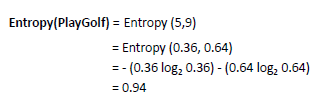
\includegraphics[width=0.8\linewidth,keepaspectratio]{dt12}
% % \end{center}
% % \end{frame}

% % %%%%%%%%%%%%%%%%%%%%%%%%%%%%%%%%%%%%%%%%%%%%%%%%%%%%%%%%%%
% % \begin{frame}[fragile]\frametitle{Step 2 (Recap)}
% % \begin{itemize}
% % \item The dataset is then split on the different attributes. 
% % \item The entropy for each branch is calculated. 
% % \item Then it is added proportionally, to get total entropy for the split. 
% % \item The resulting entropy is subtracted from the entropy before the split. 
% % \item The result is the Information Gain, or decrease in entropy
% % \end{itemize}
% % \begin{center}
% % 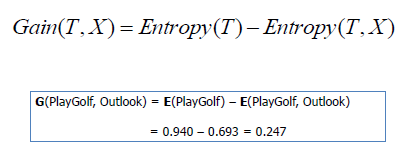
\includegraphics[width=0.5\linewidth,keepaspectratio]{dt14}

% % \end{center}
% % \end{frame}

% % %%%%%%%%%%%%%%%%%%%%%%%%%%%%%%%%%%%%%%%%%%%%%%%%%%%%%%%%%%%%%%%%%%%%%%%%%%%%%%%%%%
% % \begin{frame}[fragile]\frametitle{Step 2}
% % Calculate entropy of the target
% % \begin{center}
% % 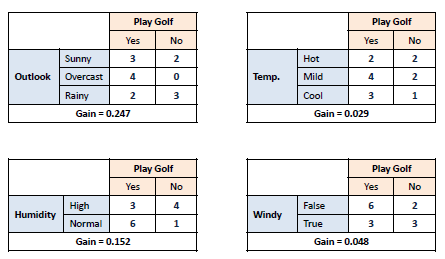
\includegraphics[width=0.8\linewidth,keepaspectratio]{dt13}
% % \end{center}
% % \end{frame}

% % %%%%%%%%%%%%%%%%%%%%%%%%%%%%%%%%%%%%%%%%%%%%%%%%%%%%%%%%%%%%%%%%%%%%%%%%%%%%%%%%%%
% % \begin{frame}[fragile]\frametitle{Step 3}
% % Choose attribute with the largest information gain

% % \begin{center}
% % 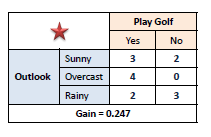
\includegraphics[width=0.4\linewidth,keepaspectratio]{dt15}

% % 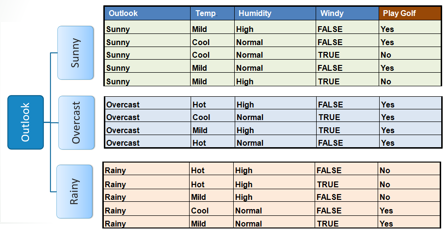
\includegraphics[width=0.7\linewidth,keepaspectratio]{dt16}
% % \end{center}
% % \end{frame}

% % %%%%%%%%%%%%%%%%%%%%%%%%%%%%%%%%%%%%%%%%%%%%%%%%%%%%%%%%%%%%%%%%%%%%%%%%%%%%%%%%%%
% % \begin{frame}[fragile]\frametitle{Step 4a}
 % % A branch with entropy of 0 is a leaf node.
 % % \begin{center}
% % 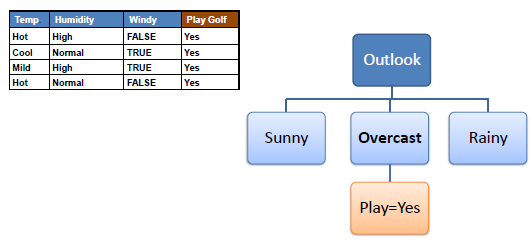
\includegraphics[width=0.8\linewidth,keepaspectratio]{dt17}
% % \end{center}
% % \end{frame}

% % %%%%%%%%%%%%%%%%%%%%%%%%%%%%%%%%%%%%%%%%%%%%%%%%%%%%%%%%%%%%%%%%%%%%%%%%%%%%%%%%%%
% % \begin{frame}[fragile]\frametitle{Step 4b}
% % A branch with entropy more than 0 needs further splitting
% % \begin{center}
% % 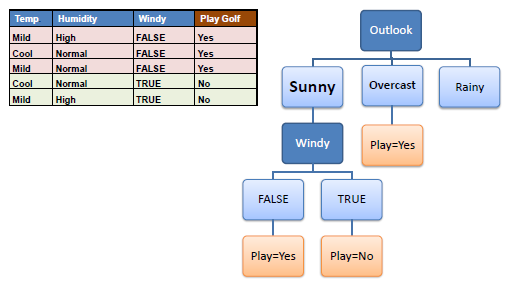
\includegraphics[width=0.8\linewidth,keepaspectratio]{dt18}
% % \end{center}
% % \end{frame}

% % %%%%%%%%%%%%%%%%%%%%%%%%%%%%%%%%%%%%%%%%%%%%%%%%%%%%%%%%%%%%%%%%%%%%%%%%%%%%%%%%%%
% % \begin{frame}[fragile]\frametitle{Step 5}
% % The ID3 algorithm is run recursively on the non-leaf branches, until all data is classified.
% % \end{frame}





% % %%%%%%%%%%%%%%%%%%%%%%%%%%%%%%%%%%%%%%%%%%%%%%%%%%%%%%%%%%%%%%%%%%%%%%%%%%%%%%%%%%
% % \begin{frame}[fragile]\frametitle{}
% % \begin{center}
% % {\Large Information Gain - Disadvantage}
% % \end{center}
% % \end{frame}



% % %%%%%%%%%%%%%%%%%%%%%%%%%%%%%%%%%%%%%%%%%%%%%%%%%%%%%%%%%%
% % \begin{frame}[fragile]\frametitle{Information Gain Problem}
% % \begin{itemize}
% % \item Say, if we split our John-Plays-Tennis example on Day, then there will be 14 partitions.
% % \item Each partition will have either Yes or No (just one answer possible)
% % \item So, all the leaves are Pure.
% % \item Here information gain is good, as  splitting on Day gave us perfect answer within one split.
% % \item But 14 partitions are too much, right?
% % \end{itemize}

% % \begin{center}
% % 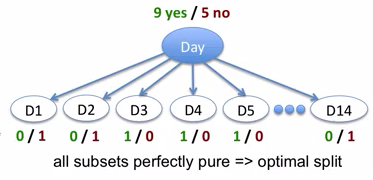
\includegraphics[width=0.5\linewidth,keepaspectratio]{split1}
% % \end{center}

% % \end{frame}

% % %%%%%%%%%%%%%%%%%%%%%%%%%%%%%%%%%%%%%%%%%%%%%%%%%%%%%%%%%%
% % \begin{frame}[fragile]\frametitle{Information Gain Problem}
% % \begin{itemize}
% % \item Problem with splitting on Day, is what do you predict for Day 15??
% % \item You just don't have a branch.
% % \item Such values would be there in dataset, and Information Gain will bring them forward for splitting first
% % \item To avoid this bias, we need to normalize the Information Gain.
% % \item Its called Intrinsic Information or Split Entropy.
% % \item It basically says, that if this partitioning is resulting into too tiny subsets or not.
% % \end{itemize}
% % $InformationGain = Entropy(s) - \sum \frac{s_i}{s} E(s_i) = 0.94$

% % \end{frame}

% % %%%%%%%%%%%%%%%%%%%%%%%%%%%%%%%%%%%%%%%%%%%%%%%%%%%%%%%%%%
% % \begin{frame}[fragile]\frametitle{Intrinsic Information}
% % \begin{itemize}
% % \item The intrinsic information represents the potential information generated by splitting the dataset By A's values
% % $IntrinsicInfor(S,A) = - \sum_{i=v \in Values(A)} (s_i/s) log(s_i/s)$
% % \item $A$: Candidate Attribute
% % \item $v$: Possible values of A
% % \item $s$: Set of all examples
% % \item $s_i$: Subset where $X_A = v$
% % \end{itemize}

% % $IntrinsicInfor(S,A) = - \sum_{i=v \in Values(A)} (1/14) log(1/14) = 3.807$

% % Attributes with higher intrinsic information are less useful (how? see next \ldots)
% % \end{frame}

% % %%%%%%%%%%%%%%%%%%%%%%%%%%%%%%%%%%%%%%%%%%%%%%%%%%%%%%%%%%
% % \begin{frame}[fragile]\frametitle{Information Gain Ratio}
% % \begin{itemize}
% % \item Gain ratio takes  into account number and size of branches when choosing an attribute
% % \item It corrects the information gain by taking the intrinsic information into account
% % \item It penalizes attributes with many values
% % \item Gain ratio (Quinlan'86) normalizes Info Gain by Intrinsic Info
% % $GainRatio(S,A) = \frac{InfomrationGain(S,A)}{IntrinsicInfor(S,A)}$
% % \item  $GainRatio(S,A) = \frac{0.940}{3.807} = 0.246$
% % \end{itemize}
% % \end{frame}

% %%%%%%%%%%%%%%%%%%%%%%%%%%%%%%%%%%%%%%%%%%%%%%%%%%%%%%%%%%%
% %\begin{frame}[fragile]\frametitle{Information Gain Example}
% %\begin{center}
% %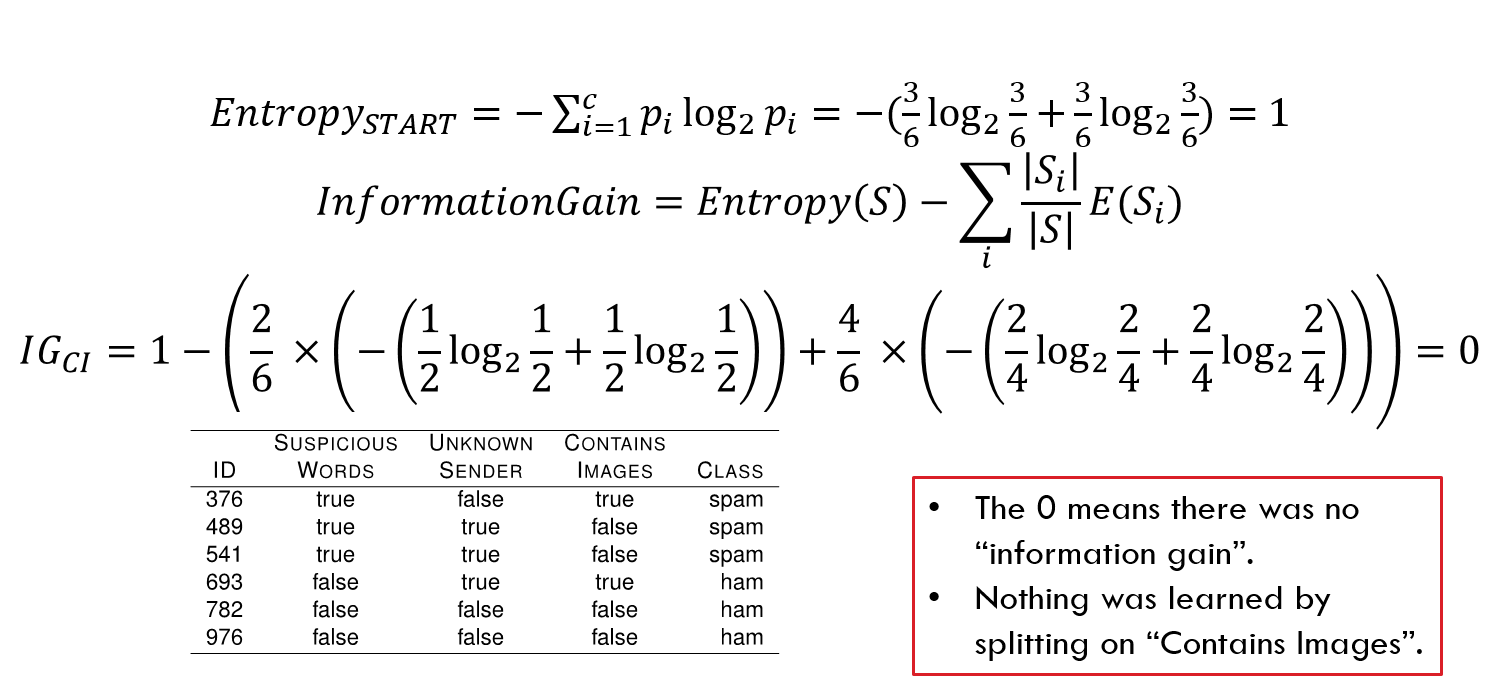
\includegraphics[width=\linewidth,keepaspectratio]{infogain}
% %\end{center}
% %\end{frame}
% %
% %%%%%%%%%%%%%%%%%%%%%%%%%%%%%%%%%%%%%%%%%%%%%%%%%%%%%%%%%%%
% %\begin{frame}[fragile]\frametitle{Calculate the Information Gain on Each Feature}
% %\begin{center}
% %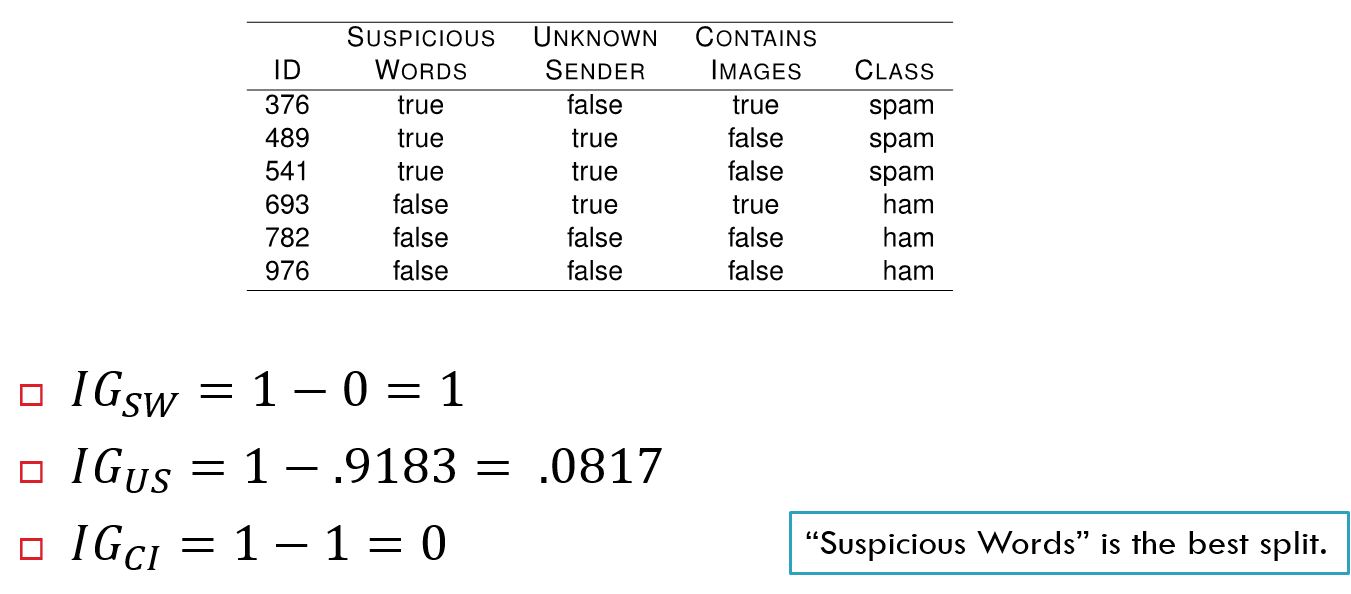
\includegraphics[width=\linewidth,keepaspectratio]{calcgain}
% %\end{center}
% %\end{frame}

%%%%%%%%%%%%%%%%%%%%%%%%%%%%%%%%%%%%%%%%%%%%%%%%%%%%%%%%%%%%%%%%%%%%%%%%%%%%%%%%%%
\begin{frame}[fragile]\frametitle{}
\begin{center}
{\Large GINI Index}
\end{center}

{\tiny (Ref: Decision Tree. It begins here - Rishabh Jain)}

\end{frame}

%%%%%%%%%%%%%%%%%%%%%%%%%%%%%%%%%%%%%%%%%%%%%%%%%%%%%%%%%%
\begin{frame}[fragile]\frametitle{Gini Index}
Gini index says, if we select two items from a population at random then they must be of same class and probability for this is 1 if population is pure.
\begin{itemize}
\item Works with categorical target variable
\item Performs only Binary splits
\item Higher the value of Gini higher the homogeneity
\item CART (Classification and Regression Tree) uses Gini method to create binary splits
\end{itemize}
\end{frame}

%%%%%%%%%%%%%%%%%%%%%%%%%%%%%%%%%%%%%%%%%%%%%%%%%%%%%%%%%%
\begin{frame}[fragile]\frametitle{Gini Index Steps}
Steps to Calculate Gini for a split
\begin{itemize}
\item Calculate Gini for sub-nodes, using formula sum of square of probability for success and failure $(p^2 + q^2)$
\item Calculate Gini for split using weighted Gini score of each node of that split
\end{itemize}
\end{frame}

%%%%%%%%%%%%%%%%%%%%%%%%%%%%%%%%%%%%%%%%%%%%%%%%%%%%%%%%%%
\begin{frame}[fragile]\frametitle{Example}
\begin{itemize}
\item We want to segregate the students based on target variable ( playing cricket or not )
\item We split the population using two input variables Gender and Class. 
\item Now, I want to identify which split is producing more homogeneous sub-nodes using Gini index.
\end{itemize}
\end{frame}

%%%%%%%%%%%%%%%%%%%%%%%%%%%%%%%%%%%%%%%%%%%%%%%%%%%%%%%%%%
\begin{frame}[fragile]\frametitle{Entropy}
\begin{center}
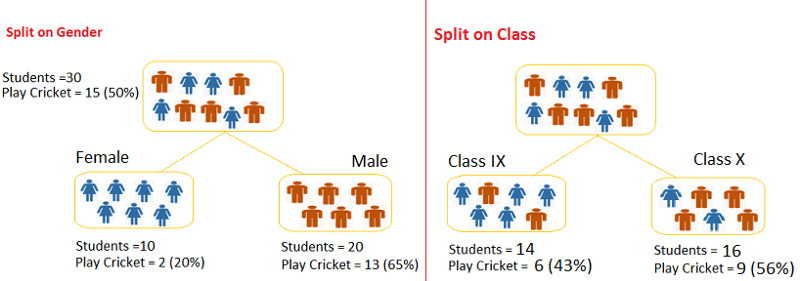
\includegraphics[width=\linewidth,keepaspectratio]{dt19}
\end{center}

(Note:characters shown in the box are not proportional to numbers shown outside!!!)
\end{frame}

%%%%%%%%%%%%%%%%%%%%%%%%%%%%%%%%%%%%%%%%%%%%%%%%%%%%%%%%%%
\begin{frame}[fragile]\frametitle{Split on Gender}
\begin{itemize}
\item Gini for sub-node Female $= (0.2)*(0.2)+(0.8)*(0.8)=0.68$
\item Gini for sub-node Male $= (0.65)*(0.65)+(0.35)*(0.35)=0.55$
\item Weighted Gini for Split Gender $= (10/30)*0.68+(20/30)*0.55 = 0.59$
\end{itemize}
\begin{center}
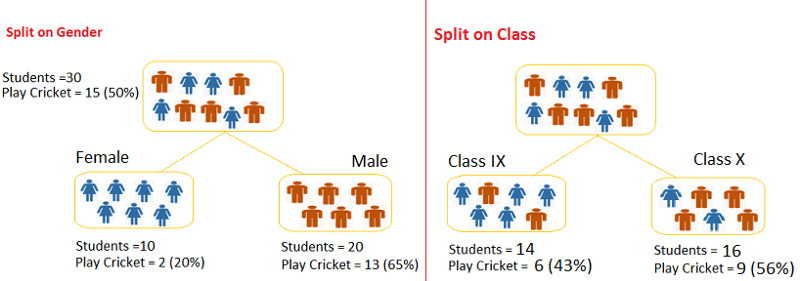
\includegraphics[width=0.6\linewidth,keepaspectratio]{dt19}
\end{center}
\end{frame}

%%%%%%%%%%%%%%%%%%%%%%%%%%%%%%%%%%%%%%%%%%%%%%%%%%%%%%%%%%
\begin{frame}[fragile]\frametitle{Split on Class}
\begin{itemize}
\item Gini for sub-node Class IX $= (0.43)*(0.43)+(0.57)*(0.57)=0.51$
\item Gini for sub-node Class X $= (0.56)*(0.56)+(0.44)*(0.44)=0.51$
\item Weighted Gini for Split Class $= (14/30)*0.51+(16/30)*0.51 = 0.51$
\end{itemize}
Above, you can see that Gini score for Split on Gender is higher than Split on Class, hence, the node split will take place on Gender.
\end{frame}

%%%%%%%%%%%%%%%%%%%%%%%%%%%%%%%%%%%%%%%%%%%%%%%%%%%%%%%%%%
\begin{frame}[fragile]\frametitle{GINI Index (Recap)}
A measure of inequality developed by an Italian named Gini.
\begin{itemize}
\item Definition : Expected error rate
$G(S) = 1 - [\sum p(j|t)^2]$
\item GINI =0 (All elements are same class)
\item  GINI =0.5 (All elements evenly split between classes)
\end{itemize}
\begin{center}
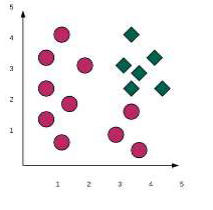
\includegraphics[width=0.3\linewidth,keepaspectratio]{gini1}
\end{center}

$G(t) = 1 - [(\frac{10}{16})^2 + (\frac{6}{16})^2] = 0.46875$
\end{frame}

%%%%%%%%%%%%%%%%%%%%%%%%%%%%%%%%%%%%%%%%%%%%%%%%%%%%%%%%%%
\begin{frame}[fragile]\frametitle{GINI Gain (Recap)}
\begin{itemize}
\item Definition :
$G(A,S) = G(S) - \sum (s_j/s)G(S)$
\item If we Split $X < 4$
\item   $Gini < 4 = 0.4081$
\item $Gini > 4 = 0$
\item Gini Gain = 0.4687 - 10/16 (0.4081) - (0/16) (0)
\item Gini Gain = 0.2136
\end{itemize}
\begin{center}
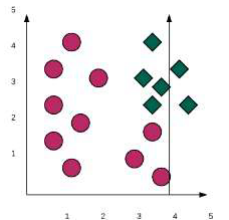
\includegraphics[width=0.3\linewidth,keepaspectratio]{gini2}
\end{center}

\end{frame}


%%%%%%%%%%%%%%%%%%%%%%%%%%%%%%%%%%%%%%%%%%%%%%%%%%%%%%%%%%
\begin{frame}[fragile]\frametitle{When to use which?}
\begin{itemize}
\item  Gini for continuous attributes
\item   Entropy for categorical.
\item  Entropy is slower to calculate than GINI
\item  Gini may fail with very small probability
\item  Difference between the two is theoretically around 2\%
\end{itemize}
%$InformationGain = Entropy(s) - \sum \frac{s_i}{s} E(s_i)$
\end{frame}

%
%%%%%%%%%%%%%%%%%%%%%%%%%%%%%%%%%%%%%%%%%%%%%%%%%%%%
%\begin{frame}[fragile]\frametitle{Comparison}
%
%\adjustbox{valign=t}{
%\begin{minipage}{0.45\linewidth}
%Advantages
%\begin{itemize}
%\item Trees are very easy to explain. Easier to explain than linear regression
%\item Trees can be displayed graphically and interpreted by a non-expert
%\item Decision trees may more closely mirror human decision-making
%%\item Trees can easily handle qualitative predictors. 
%%No dummy variables
%\end{itemize}
%
%\end{minipage}
%}
%\hfill
%\adjustbox{valign=t}{
%\begin{minipage}{0.45\linewidth}
%Disadvantages
%\begin{itemize}
%\item Trees usually do not have same level of predictive accuracy as other data mining algorithms
%\item But, predictive performance of decision trees can be improved by aggregating trees.
%\item Techniques: bagging, boosting, random forests
%\end{itemize}
%
%\end{minipage}
%}
%\end{frame}

%%%%%%%%%%%%%%%%%%%%%%%%%%%%%%%%%%%%%%%%%%%%%%%%%%%%%%%%%%%%%%%%%%%%%%%%%%%%%%%%%%
\begin{frame}[fragile]\frametitle{}
\begin{center}
{\Large Over-fitting of Trees}
\end{center}
\end{frame}

%%%%%%%%%%%%%%%%%%%%%%%%%%%%%%%%%%%%%%%%%%%%%%%%%%%%%%%%%%
\begin{frame}[fragile]\frametitle{Overfitting Example}
\begin{center}
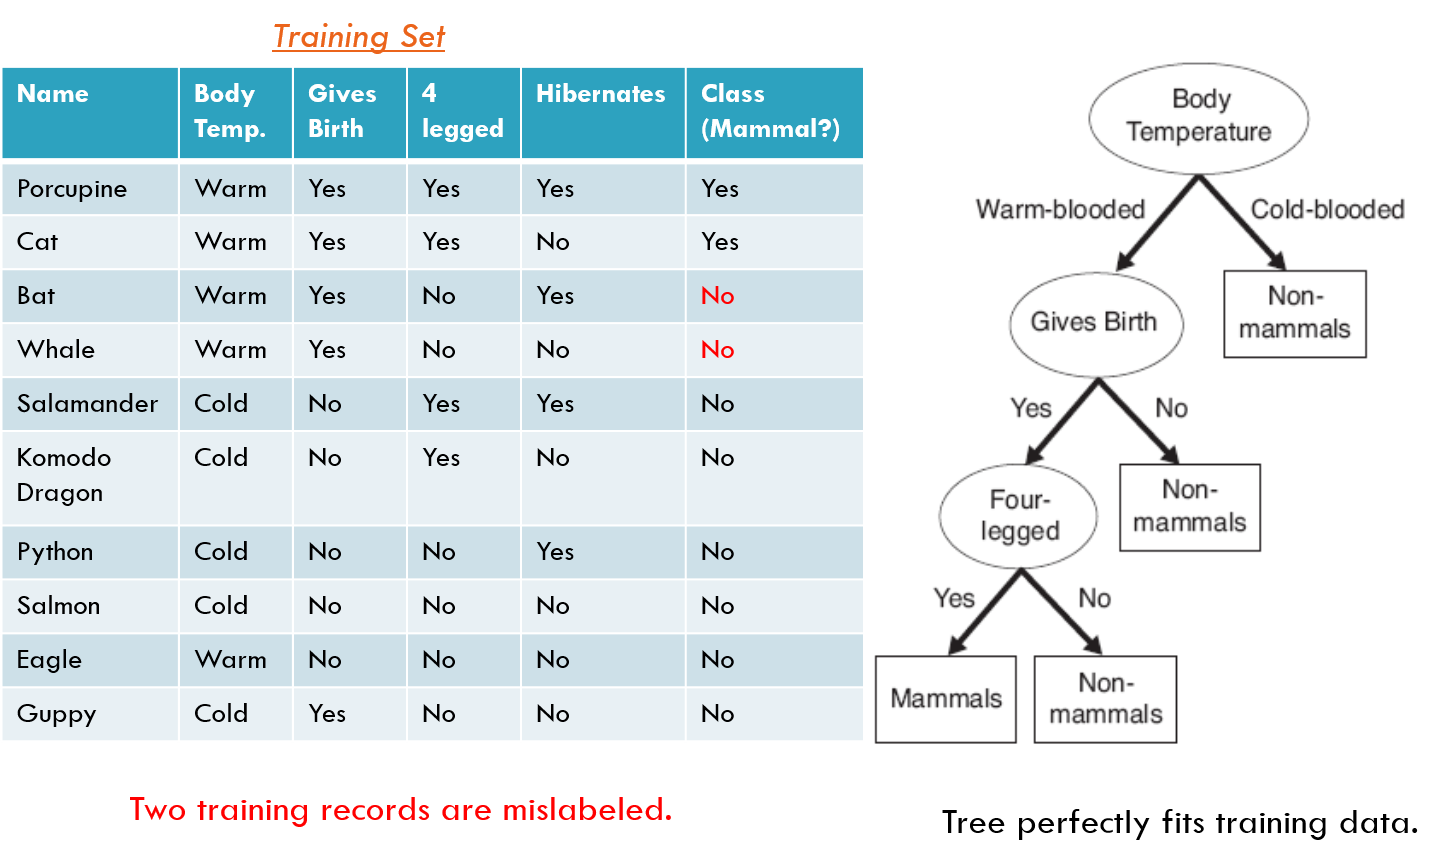
\includegraphics[width=\linewidth,keepaspectratio]{ovex1}
\end{center}
\end{frame}

%%%%%%%%%%%%%%%%%%%%%%%%%%%%%%%%%%%%%%%%%%%%%%%%%%%%%%%%%%
\begin{frame}[fragile]\frametitle{Overfitting Example}
\begin{center}
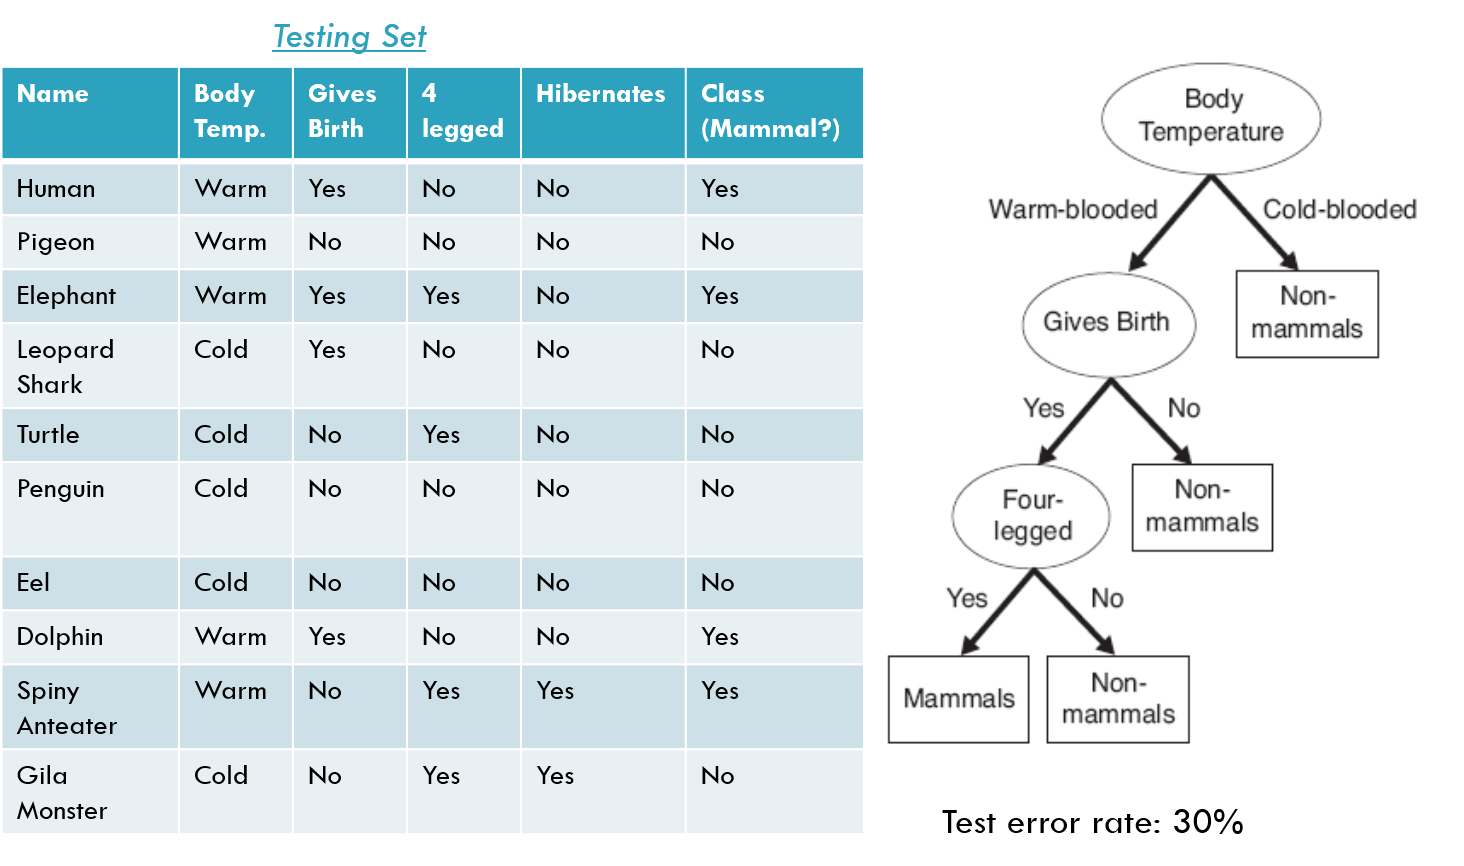
\includegraphics[width=\linewidth,keepaspectratio]{ovex2}
\end{center}
\end{frame}

%%%%%%%%%%%%%%%%%%%%%%%%%%%%%%%%%%%%%%%%%%%%%%%%%%%%%%%%%%
\begin{frame}[fragile]\frametitle{Overfitting Example}
\begin{center}
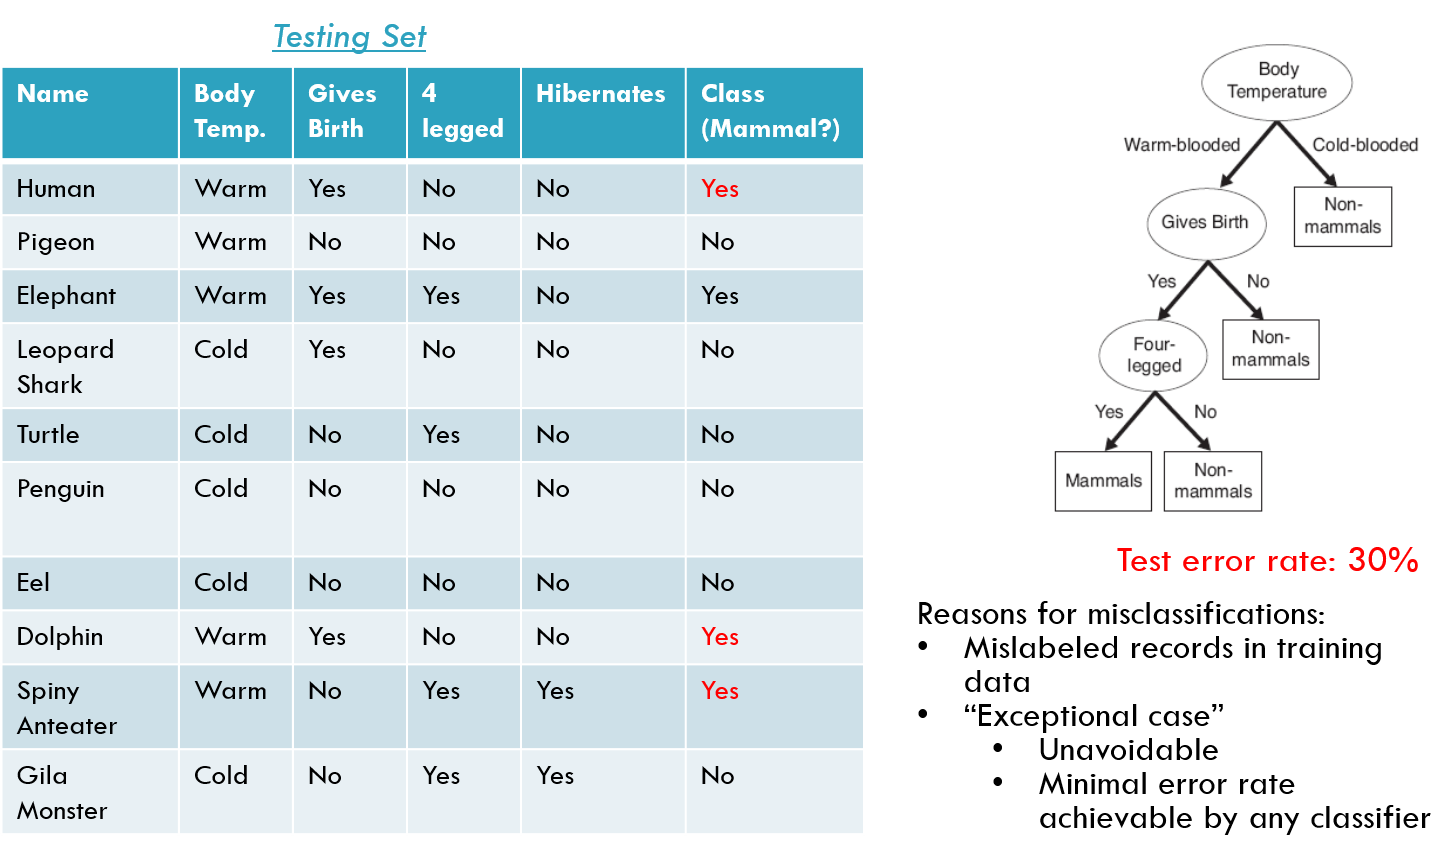
\includegraphics[width=\linewidth,keepaspectratio]{ovex3}
\end{center}
\end{frame}

%%%%%%%%%%%%%%%%%%%%%%%%%%%%%%%%%%%%%%%%%%%%%%%%%%%%%%%%%%
\begin{frame}[fragile]\frametitle{Overfitting Example}
\begin{center}
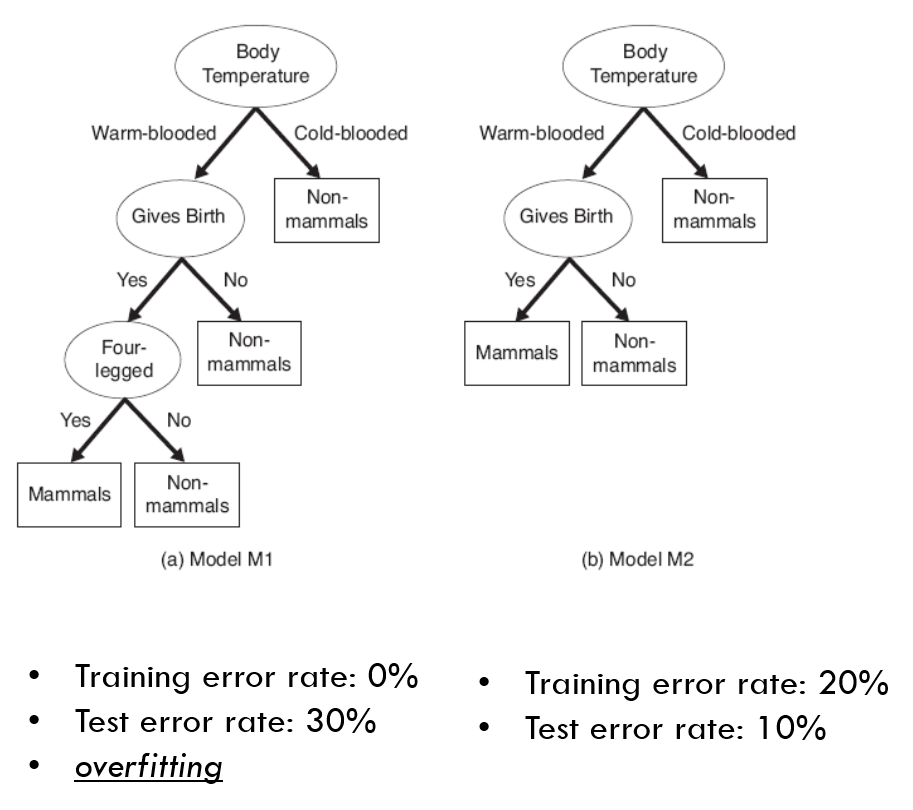
\includegraphics[width=\linewidth,keepaspectratio]{ovex4}
\end{center}
\end{frame}


%%%%%%%%%%%%%%%%%%%%%%%%%%%%%%%%%%%%%%%%%%%%%%%%%%%%%%%%%%
\begin{frame}[fragile]\frametitle{Over-fitting and Decision Trees}
\begin{itemize}
\item Tree tries to reach till you get to all pure nodes, however unusual they are. These unusual points may not be there in the test sets or in general.
\item The likelihood of over-fitting occurring increases as a tree gets deeper. 
\item Whats the way to detect?
\end{itemize}
\end{frame}


%%%%%%%%%%%%%%%%%%%%%%%%%%%%%%%%%%%%%%%%%%%%%%%%%%%%%%%%%%%%%%%%%%%%%%%%
\begin{frame}[fragile]\frametitle{Detection}
Roughly speaking, over-fitting typically occurs when the ratio $\frac{ComplexityOfTheModel}{TrainingSize}$ is too high.

\begin{center}
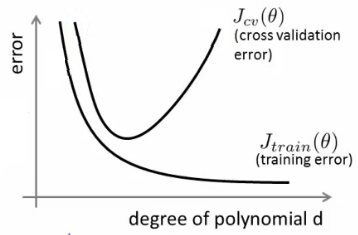
\includegraphics[width=0.4\linewidth,keepaspectratio]{ovefit1}
\end{center}
	\begin{itemize}
	\item If your data is in two dimensions, you have 10000 points in the training set and the model is a line, you are likely to under-fit.
	\item If your data is in two dimensions, you have 10 points in the training set and the model is 100-degree polynomial, you are likely to over-fit. 
	\end{itemize}
	
(Ref:Why Is Overfitting Bad in Machine Learning? - StackOverflow)
\end{frame}

%%%%%%%%%%%%%%%%%%%%%%%%%%%%%%%%%%%%%%%%%%%%%%%%%%%%%%%%%%%%%%%%%%%%%%%%
\begin{frame}[fragile]\frametitle{Solution}

\begin{center}
\includegraphics[width=0.4\linewidth,keepaspectratio]{ovefit2}
\end{center}

	\begin{itemize}
	\item In many texts, ``iterations'' is used on X axis, which is easy to imagine in case of Neural Networks, where each epoch refines model by fitting better question/weights.
	\item In case of Machine Learning, there no iterations. How to detect Over-fitting in case of Decision Tree?
	\item Initially when, tree is small it has not fit the data yet, so its under fitting phase. Losses are HIGH for both, training as well as testing (validation)
	\item As more levels get added in tree or more degrees in polynomial regression, under-fitting reduces and losses come down.
	\item At one point, training loss still reduces but validation loss starts jumping up. Thats over-fitting. Model is fitting training data TOO tightly and is OFF the validation data.
	\end{itemize}
	
(Ref:Why Is Over-fitting Bad in Machine Learning? - StackOverflow)
\end{frame}


% %%%%%%%%%%%%%%%%%%%%%%%%%%%%%%%%%%%%%%%%%%%%%%%%%%%%%%%%%%
% \begin{frame}[fragile]\frametitle{Detecting Over-fitting, based on Target distribution}
% \begin{itemize}
% \item With iterations on x axis and error or loss on y, if training set is coming down and validation set is going up (after a while) then its a over-fit.
% \item Tree is built to fullest with training set and does not work well on validation set and thus error-ing out more.
% \end{itemize}
% \begin{center}
% \includegraphics[width=0.6\linewidth,keepaspectratio]{dt20}
% \end{center}
% \end{frame}


% %%%%%%%%%%%%%%%%%%%%%%%%%%%%%%%%%%%%%%%%%%%%%%%%%%%%%%%%%%
% \begin{frame}[fragile]\frametitle{Detecting Over-fitting, based on Target distribution}
% Solution : Cross Validation
% \begin{itemize}
% \item Split training data into two parts, say 70\% and 30\%.
% \item Just one split is not good as distribution of features in training and test sets could be different. 
% \item Need multiple, random , all encompassing splits, like done by K-Fold.
% \item As the model is seeing all parts of training and validation, it is more and chances of over-fitting are less.
% \end{itemize}
% \end{frame}




%%%%%%%%%%%%%%%%%%%%%%%%%%%%%%%%%%%%%%%%%%%%%%%%%%%%%%%%%%
\begin{frame}[fragile]\frametitle{Over-fitting and Decision Trees}
Solution : Pruning
\begin{itemize}
\item Tree pruning identifies and removes subtrees within a decision tree that are likely to be due to noise and sample variance in the training set used to induce it.
\item Pruning will result in decision trees being created that are not consistent with the training set used to build them.
\item But we are more interested in created prediction models that generalize well to new data! 
\item Solutions: Pre-pruning (Early Stopping), Post-pruning
\end{itemize}
\end{frame}

%%%%%%%%%%%%%%%%%%%%%%%%%%%%%%%%%%%%%%%%%%%%%%%%%%%%%%%%%%
\begin{frame}[fragile]\frametitle{Pre-pruning Techniques}
\begin{itemize}
\item Stop creating subtrees when the number of instances in a partition falls below a threshold
\item Information gain measured at a node is not deemed to be sufficient to make partitioning the data worthwhile
\item Depth of the tree goes beyond a predefined limit
\item Benefits: Computationally efficient; works well for small datasets.
\item Downsides: Stopping too early will fail to create the most effective trees.
\end{itemize}
\end{frame}

%%%%%%%%%%%%%%%%%%%%%%%%%%%%%%%%%%%%%%%%%%%%%%%%%%%%%%%%%%
\begin{frame}[fragile]\frametitle{Post-pruning Techniques}
\begin{itemize}
\item Decision tree initially grown to its maximum size
\item Then examine each branch
\item Branches that are deemed likely to be due to over-fitting are pruned.
\item Post-pruning tends to give better results than pre-pruning
\item Which is faster? Post-pruning is more computationally expensive than pre-pruning because entire tree is grown
\item Techniques: Reduced Error Pruning;
Cost Complexity Pruning

\end{itemize}
\end{frame}


%%%%%%%%%%%%%%%%%%%%%%%%%%%%%%%%%%%%%%%%%%%%%%%%%%%%%%%%%%%
%\begin{frame}[fragile]\frametitle{Reduced Error Pruning}
%\begin{itemize}
%\item Starting at the leaves, each node is replaced with its most popular class.
%\item If the accuracy is not affected, then the change is kept.
%\item Evaluate accuracy on a validation set
%\item Set aside some of the training set as a validation set
%\item Advantages: simplicity and speed
%
%\end{itemize}
%\end{frame}
%
%%%%%%%%%%%%%%%%%%%%%%%%%%%%%%%%%%%%%%%%%%%%%%%%%%%%%%%%%%%
%\begin{frame}[fragile]\frametitle{Cost Complexity Pruning}
%\begin{itemize}
%\item Nonnegative tuning parameter: $\alpha$; ``Penalizing cost'' / ``complexity parameter''
%\item Will look at different pruned subtrees and compare their performance on a test sample
%\item $\alpha$ determines the trade-off between misclassification error and the model complexity
%\item Small $\alpha$: penalty for larger tree is small
%\item Larger $\alpha$: smaller trees preferred depending on \# of errors
%
%\end{itemize}
%\end{frame}


%%%%%%%%%%%%%%%%%%%%%%%%%%%%%%%%%%%%%%%%%%%%%%%%%%%%%%%%%%%
%\begin{frame}[fragile]\frametitle{Post-Pruning Example}
%Example validation set:
%
%
%\begin{center}
%\includegraphics[width=\linewidth,keepaspectratio]{postprunex}
%\end{center}
%Induced decision tree from training data
%Need to prune?
%
%\end{frame}
%
%%%%%%%%%%%%%%%%%%%%%%%%%%%%%%%%%%%%%%%%%%%%%%%%%%%%%%%%%%%
%\begin{frame}[fragile]\frametitle{Post-Pruning Example}
%Pruned nodes in black
%
%
%
%\begin{center}
%\includegraphics[width=\linewidth,keepaspectratio]{postprunex1}
%\end{center}
%
%\end{frame}


%%%%%%%%%%%%%%%%%%%%%%%%%%%%%%%%%%%%%%%%%%%%%%%%%%%%%%%%%%%
%\begin{frame}[fragile]\frametitle{Building a Decision Tree w/ Pruning}
%\begin{itemize}
%\item Use k-fold (10-fold) cross-validation to choose $\alpha$
%\begin{itemize}
%\item Fully grow a tree using the 90\% training set
%\item Apply cost complexity pruning using different $\alpha$ parameters
%\item Evaluate each pruned tree using the 10\% testing set
%\end{itemize}
%\item Average results over each fold find the $\alpha$ that minimizes error
%\item Fully grow a large tree on the training data
%\item Apply cost complexity pruning with the found $\alpha$parameter to the large tree, to obtain the ``best'' subtree
%\end{itemize}
%\end{frame}
%
%
%%%%%%%%%%%%%%%%%%%%%%%%%%%%%%%%%%%%%%%%%%%%%%%%%%%%%%%%%%%
%\begin{frame}[fragile]\frametitle{Occam's Razor}
%\begin{itemize}
%\item General Principle (Occam's Razor): given two models with same generalization (testing) errors, the simpler model is preferred over the more complex model
%
%\item Additional components in a more complex model have greater chance at being fitted purely by chance
%
%\item Problem solving principle by philosopher William of Ockham (1287-1347)
%
%\end{itemize}
%\end{frame}

%%%%%%%%%%%%%%%%%%%%%%%%%%%%%%%%%%%%%%%%%%%%%%%%%%%%%%%%%%%%%%%%%%%%%%%%%%%%%%%%%%
\begin{frame}[fragile]\frametitle{}
\begin{center}
{\Large Decision Trees for Regression}
\end{center}
\end{frame}


%%%%%%%%%%%%%%%%%%%%%%%%%%%%%%%%%%%%%%%%%%%%%%%%%%%%%%%%%%
\begin{frame}[fragile]\frametitle{Regression Trees}
\begin{itemize}
\item Target Attribute:

\begin{itemize}
\item Decision (Classification) Trees: qualitative
\item Regression Trees: continuous
\end{itemize}
\item Decision trees: reduce the entropy in each subtree
\item Regression trees: reduce the variance in each subtree
\item Idea: adapt ID3 algorithm measure of Information Gain to use variance rather than node impurity
\end{itemize}
\end{frame}


%%%%%%%%%%%%%%%%%%%%%%%%%%%%%%%%%%%%%%%%%%%%%%%%%%%%%%%%%%
\begin{frame}[fragile]\frametitle{Regression Trees}
When predicting a numeric variable, the idea of a tree construction remains the same, but the quality criteria changes.
Variance around the mean:

$\Large D = \frac{1}{\ell} \sum\limits_{i =1}^{\ell} (y_i - \frac{1}{\ell} \sum\limits_{i =1}^{\ell} y_i)^2,$

where $\ell$ is the number of samples in a leaf,  $y_i$  is the value of the target variable. Simply put, by minimizing the variance around the mean, we look for features that divide the training set in such a way that the values of the target feature in each leaf are roughly equal.

{\tiny (Ref: https://www.kaggle.com/kashnitsky/topic-3-decision-trees-and-knn )}

\end{frame}


%%%%%%%%%%%%%%%%%%%%%%%%%%%%%%%%%%%%%%%%%%%%%%%%%%%%%%%%%%
\begin{frame}[fragile]\frametitle{Regression Trees Example}
Let's generate some data distributed by the function $f(x) = e^{-x ^ 2} + 1.5 * e^{-(x - 2) ^ 2}$
  with some noise. Then we will train a tree on it and show what predictions it makes.


{\tiny (Ref: https://www.kaggle.com/kashnitsky/topic-3-decision-trees-and-knn )}

\end{frame}

%%%%%%%%%%%%%%%%%%%%%%%%%%%%%%%%%%%%%%%%%%%%%%%%%%%%%%%%%%
\begin{frame}[fragile]\frametitle{Regression Trees Example}
\begin{lstlisting}
n_train = 150        
n_test = 1000       
noise = 0.1

def f(x):
    x = x.ravel()
    return np.exp(-x ** 2) + 1.5 * np.exp(-(x - 2) ** 2)

def generate(n_samples, noise):
    X = np.random.rand(n_samples) * 10 - 5
    X = np.sort(X).ravel()
    y = np.exp(-X ** 2) + 1.5 * np.exp(-(X - 2) ** 2) + \
    np.random.normal(0.0, noise, n_samples)
    X = X.reshape((n_samples, 1))
    return X, y

X_train, y_train = generate(n_samples=n_train, noise=noise)
X_test, y_test = generate(n_samples=n_test, noise=noise)
\end{lstlisting}

{\tiny (Ref: https://www.kaggle.com/kashnitsky/topic-3-decision-trees-and-knn )}

\end{frame}

%%%%%%%%%%%%%%%%%%%%%%%%%%%%%%%%%%%%%%%%%%%%%%%%%%%%%%%%%%
\begin{frame}[fragile]\frametitle{Regression Trees Example}
\begin{lstlisting}
from sklearn.tree import DecisionTreeRegressor

reg_tree = DecisionTreeRegressor(max_depth=5, random_state=17)

reg_tree.fit(X_train, y_train)
reg_tree_pred = reg_tree.predict(X_test)

plt.figure(figsize=(10, 6))
plt.plot(X_test, f(X_test), "b")
plt.scatter(X_train, y_train, c="b", s=20)
plt.plot(X_test, reg_tree_pred, "g", lw=2)
plt.xlim([-5, 5])
plt.title("Decision tree regressor, MSE = %.2f" % np.sum((y_test - reg_tree_pred) ** 2))
plt.show()
\end{lstlisting}

{\tiny (Ref: https://www.kaggle.com/kashnitsky/topic-3-decision-trees-and-knn )}

\end{frame}


%%%%%%%%%%%%%%%%%%%%%%%%%%%%%%%%%%%%%%%%%%%%%%%%%%%%%%%%%%%%%%%%%%%%%%%%
\begin{frame}[fragile]\frametitle{Binary outcome}
\begin{center}
\includegraphics[width=0.9\linewidth]{mlcourse18}
\end{center}

We see that the decision tree approximates the data with a piecewise constant function.

{\tiny (Ref: https://www.kaggle.com/kashnitsky/topic-3-decision-trees-and-knn )}

\end{frame}





%%%%%%%%%%%%%%%%%%%%%%%%%%%%%%%%%%%%%%%%%%%%%%%%%%%
\begin{frame}[fragile] \frametitle{Regression trees}
The fitting algorithm for learning such a tree is as follows:
\begin{itemize}
\item Consider splitting on every possible unique value of every
single variable in the data. Pick the `best' split from amongst
all of these options.
\item Partition the training data into two classes based on step $1$.
\item Now, iteratively apply step $1$ separately to each partition of
the data.
\item Continue splitting each subset until an appropriate
stopping criteria has been reached.
\item Calculate the mean of all the training data in a terminal node
(i.e., `leaf') of the learned tree structure. Use this as the predicted
value for future inputs that fall within the same bucket.
\end{itemize}
\end{frame}

%%%%%%%%%%%%%%%%%%%%%%%%%%%%%%%%%%%%%%%%%%%%%%%%%%%
\begin{frame}[fragile] \frametitle{Stopping criterion}
There are many commonly used stopping criterion, often used
simultaneously (if any is satisfied stop splitting the partition):
\begin{itemize}
\item minimum number of training samples in a node
\item maximum number of splits
\item minimum improvement in the best split
\item maximum depth of the tree
\end{itemize}
In practice, particularly for larger datasets, the maximum number
of splits is the mostly commonly used.
\end{frame}

%%%%%%%%%%%%%%%%%%%%%%%%%%%%%%%%%%%%%%%%%%%%%%%%%%%
\begin{frame}[fragile]\frametitle{Regression Tree Splits}

\adjustbox{valign=t}{
\begin{minipage}{0.45\linewidth}
Classification Trees

\begin{itemize}
\item Gain: ``goodness of the split''
\item larger gain = better split (better test condition)
%\begin{center}
%\includegraphics[width=\linewidth,keepaspectratio]{regrtree1}
%\end{center}

\end{itemize}

\end{minipage}
}
\hfill
\adjustbox{valign=t}{
\begin{minipage}{0.45\linewidth}
Regression Trees

\begin{itemize}
\item Impurity (variance) at a node:
\item Select feature to split on that minimizes the weighted variance across all resulting partitions:
%\begin{center}
%\includegraphics[width=\linewidth,keepaspectratio]{regrtree2}
%\end{center}

\end{itemize}

\end{minipage}
}
\end{frame}
%
%
%%%%%%%%%%%%%%%%%%%%%%%%%%%%%%%%%%%%%%%%%%%%%%%%%%%%%%%%%%%
%\begin{frame}[fragile]\frametitle{Example}
%\begin{center}
%\includegraphics[width=\linewidth,keepaspectratio]{regrex}
%\end{center}
%
%\end{frame}
%
%%%%%%%%%%%%%%%%%%%%%%%%%%%%%%%%%%%%%%%%%%%%%%%%%%%%
%\begin{frame}[fragile] \frametitle{Why trees?}
%\begin{itemize}
%\item able to interpret the important variables in a model
%\item handles missing values well in both training and testing data
%\item reasonably fast to train
%\item does not depend on the scale of the predictor variables
%\item can handle multiclass problems directly
%\item works natively with categorical variables
%\item easily modified to be robust to outliers (just replace MSE with MAD
%for evaluating splits; means with medians for predictions in terminal nodes)
%\item very fast to classify new points
%\item robust to tuning parameters (the stopping criteria), \textit{for a given set of data}
%\end{itemize}
%\end{frame}
%
%%%%%%%%%%%%%%%%%%%%%%%%%%%%%%%%%%%%%%%%%%%%%%%%%%%%
%\begin{frame}[fragile] \frametitle{Stability}
%Regression and classification trees are robust to the stopping criterion,
%but very sensitive to the input data used from training. Removing some
%small fraction, say 10\%, of the training data can often lead to an
%extremely different set of predictions.
%
%Fortunately, we can use this instability to our advantage!
%\end{frame}
%
%
%
%%%%%%%%%%%%%%%%%%%%%%%%%%%%%%%%%%%%%%%%%%%%%%%%%%%%%%%%%%%%%%%%%%%%%%%%%%%%%%%%%%
\begin{frame}[fragile]\frametitle{}
\begin{center}
{\Large Decision Tree Algorithms}
\end{center}
\end{frame}


%%%%%%%%%%%%%%%%%%%%%%%%%%%%%%%%%%%%%%%%%%%%%%%%%%%
\begin{frame}[fragile] \frametitle{Types of Decision Tree Algorithms: ID3}
\begin{itemize}
\item ID3 or Iterative Dichotomizer, was the first of three Decision Tree implementations developed by Ross Quinlan
\item Uses Information Gain as splitting criterion. 
%\item Stops at Pure leaves or when Information Gain is less than threshold. 
\item It does not apply any pruning procedure
\end{itemize}
\end{frame}

%%%%%%%%%%%%%%%%%%%%%%%%%%%%%%%%%%%%%%%%%%%%%%%%%%%
\begin{frame}[fragile] \frametitle{Types of Decision Tree Algorithms: CART}
\begin{itemize}
\item CART stands for Classification and Regression Trees.
\item Uses Gini Impurity instead. 
\item Gini Impurity is a measure of the homogeneity (or ``purity'') of the nodes.
\item It constructs binary trees, namely each internal node has exactly two outgoing edges.
\item It can handle both numeric and categorical variables 
\end{itemize}
\end{frame}

%%%%%%%%%%%%%%%%%%%%%%%%%%%%%%%%%%%%%%%%%%%%%%%%%%%
\begin{frame}[fragile] \frametitle{Types of Decision Tree Algorithms: C4.5}
\begin{itemize}
\item Improved version on ID 3 by Quinlan. 
\item Uses Information Gain as splitting criterion. 
\item Accepts both continuous and discrete features;
\item Handles incomplete data points; 
\item Solves over-fitting problem by pruning
\end{itemize}
\end{frame}

%%%%%%%%%%%%%%%%%%%%%%%%%%%%%%%%%%%%%%%%%%%%%%%%%%%%%%%%%%
\begin{frame}[fragile] \frametitle{Types of Decision Tree Algorithms: Comparison}
\begin{center}
\includegraphics[width=\linewidth,keepaspectratio]{dt9}
\end{center}
\end{frame}


%%%%%%%%%%%%%%%%%%%%%%%%%%%%%%%%%%%%%%%%%%%%%%%%%%%
\begin{frame}[fragile] \frametitle{Types of Decision Tree Algorithms: C5.0}
\begin{itemize}
\item Evolution of ID3, better than C4.5
\item Uses Information Gain Ratio as splitting criterion. 
\item Handles missing values well.
\end{itemize}
\end{frame}


%%%%%%%%%%%%%%%%%%%%%%%%%%%%%%%%%%%%%%%%%%%%%%%%%%%
\begin{frame}[fragile]\frametitle{Advantages and Disadvantages of Trees}

\adjustbox{valign=t}{
\begin{minipage}{0.45\linewidth}
Advantages


\begin{itemize}
\item Trees are very easy to explain
\item Easier to explain than linear regression
\item Trees can be displayed graphically and interpreted by a non-expert
\item Decision trees may more closely mirror human decision-making
%\item Trees can easily handle qualitative predictors
%\item No dummy variables

\end{itemize}

\end{minipage}
}
\hfill
\adjustbox{valign=t}{
\begin{minipage}{0.45\linewidth}
Disadvantages


\begin{itemize}
\item Trees usually do not have same level of predictive accuracy as other data mining algorithms
\item But, predictive performance of decision trees can be improved by aggregating trees.
Techniques: bagging, boosting, random forests

\end{itemize}

\end{minipage}
}
\end{frame}


%%%%%%%%%%%%%%%%%%%%%%%%%%%%%%%%%%%%%%%%%%%%%%%%%%%%%%%%%%%
%\begin{frame}[fragile]\frametitle{Comparison of Decision Tree Algorithms}
%\begin{itemize}
%\item C4.5:
%\begin{itemize}
%\item Proprietary extension of ID3 Algorithm to handle continuous and categorical features, and missing values
%\item Sorts continuous attributes at each node
%\item Uses post-pruning to mitigate overfitting
%\item Uses information gain, gain ratio to select optimal split
%\item J48: open source implementation of the C4.5 algorithm
%\end{itemize}
%\item CART (Classification and Regression Trees):
%\begin{itemize}
%\item Restricted to binary splits
%\item Less bushy trees
%\item Uses Gini
%
%\end{itemize}
%\item Performing evaluation experiments using different models and variants helps determine which will work best for a specific problem. 
%
%\end{itemize}
%\end{frame}




%%%%%%%%%%%%%%%%%%%%%%%%%%%%%%%%%%%%%%%%%%%%%%%%%%%%%%%%%%
\begin{frame}[fragile]\frametitle{Compared to Linear Models}
\begin{center}
\includegraphics[width=\linewidth,keepaspectratio]{complin1}
\end{center}

\end{frame}

%%%%%%%%%%%%%%%%%%%%%%%%%%%%%%%%%%%%%%%%%%%%%%%%%%%%%%%%%%
\begin{frame}[fragile]\frametitle{Compared to Linear Models}
\begin{center}
\includegraphics[width=\linewidth,keepaspectratio]{complin2}
\end{center}

\end{frame}



%%%%%%%%%%%%%%%%%%%%%%%%%%%%%%%%%%%%%%%%%%%%%%%%%%%%%%%%%%%%%%%%%%%%%%%%
\begin{frame}[fragile]\frametitle{Decision Trees (Recap)}
\begin{itemize}
	\item A decision tree or a classification tree is a tree in which each internal (non-leaf) node is labeled with an input feature. 
	\item The arcs coming from a node labeled with a feature are labeled with each of the possible values of the feature.
	\item Each leaf of the tree is labeled with a class or a probability distribution over the classes.
\item For instance, in the example below, decision trees learn from data to approximate a sine curve with a set of \textit{If-Then-Else} decision rules. 
\item The deeper the tree, the more complex the decision rules and the fitter the model.
\end{itemize}
\end{frame}

%%%%%%%%%%%%%%%%%%%%%%%%%%%%%%%%%%%%%%%%%%%%%%%%%%%%%%%%%%
\begin{frame}[fragile]\frametitle{Pros and Cons of Single Decision Tree}
Pros
\begin{itemize}
\item Simple interpretations
\item Can be built quickly.
\item Does built-in Feature selection. So, if any of the features does not get used in Splitting, it is, sort-of, ignored, not selected in prediction.
\end{itemize}
Cons
\begin{itemize}
\item Small changes in data affects structure of tree
\item So, instead of single tree, a collection of Trees is preferred
\end{itemize}
Such collection is called as `Ensemble'.
\end{frame}

%%%%%%%%%%%%%%%%%%%%%%%%%%%%%%%%%%%%%%%%%%%%%%%%%%%%%%%%%%
\begin{frame}[fragile]\frametitle{Ensemble Methods}
\begin{itemize}
\item Currently using one single classifier induced from training data as our model, to predict class of test instance
\item What if we used multiple decision trees?
\item Motivation: committee of experts working together are likely to better solve a problem than a single expert
\item But no ``group think'': each model should make predictions independently of other models in the ensemble
\item In practice: methods work surprisingly well, usually greatly improve decision tree accuracy
\end{itemize}
\end{frame}

